

\chapter{Sistema de controlo e monitorização: arquitetura e modelação}


Este capítulo tem como objetivo a descrição do sistema que resultou do trabalho prático
desta dissertação. Para esse fim, cada elemento pertencente ao sistema é caracterizado de
acordo com as suas funções, especificidades e respectiva arquitetura. É também descrito como os elementos interagem entre si. Para além disso, é apresentado todo o processo de modelação do sistema tendo por base os requisitos adquiridos pelo cliente. 



%Dashboard - Interface que apresenta a informação mais importante para o utilizador de forma apelativa, tornando mais fácil a interacção e respetiva leitura


% Mockups - Design que a plataforma deverá apresentar no fim do seu desenvolvimento.



\section{Descrição global do sistema}

Este sistema tem como objetivo a supervisão remota da produção de salicornia,  permitindo não só a monitorização dos dados adquiridos pelos sensores, como também da atuação remota de determinados comandos. Neste contexto, também será possível a aquisição de imagens que possibilitará a deteção de intrusos nas quintas onde se realiza a produção desta espécie.


\begin{figure}[!htb]
	\centering
	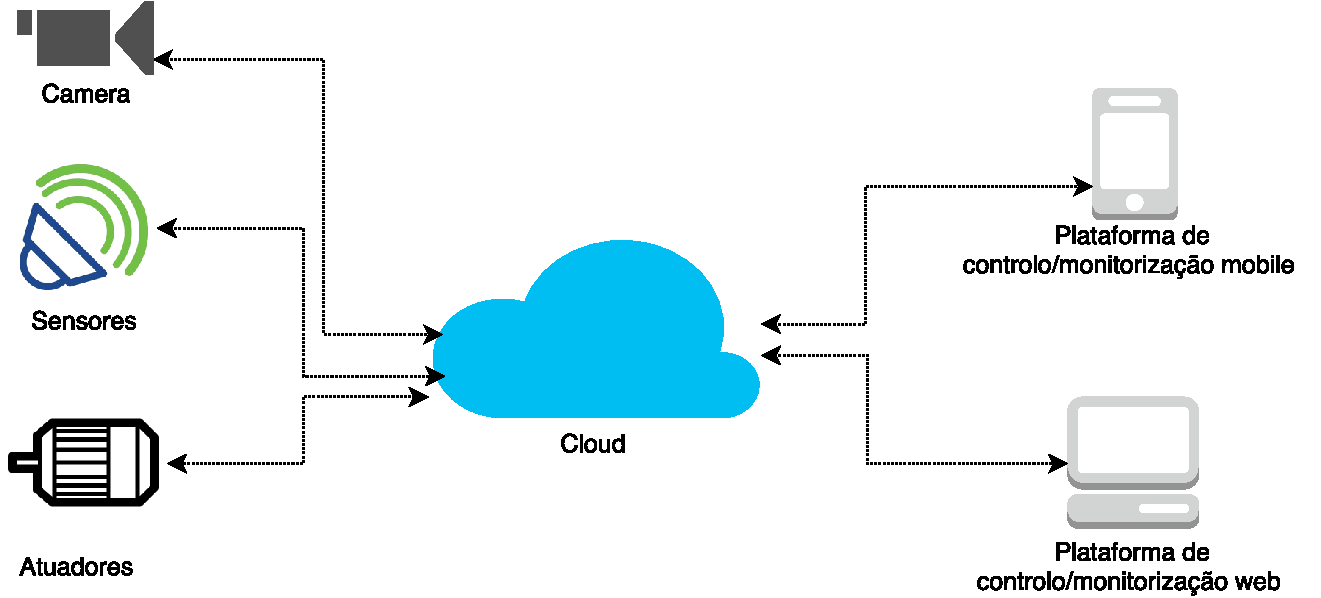
\includegraphics[scale=0.45]{esquemas/global_arquitetura.pdf}
	\caption{Ilustração principais componentes}
	\label{componentesall}
\end{figure}



O esquema da figura \ref{componentesall} ilustra de um modo geral todos os componentes e as diferentes plataformas com que o cliente pode interagir. 


Como vimos no capitulo 3, uma plantação de  Salicórnia carece de um controlo relativamente fino de certos parâmetros ambientais sobretudo da salinidade do terreno onde ela cresce. A salinidade do terreno depende, por sua vez, das chuvas, da salinidade da água dos canais da ria. Nas quintas onde se cultiva salicórnia, a produção faz-se numa espécie de leiras limitadas por pequenos canais de irrigação. Esses canais podem ser cheios de água salgada proveniente dos esteiros que rodeiam a quinta. Essa operação implica a abertura de válvulas de admissão dessa água, medida do nível da maré nos canais, monitorização da qualidade e salinidade da água exterior.



\begin{figure}[!htb]
	\centering
	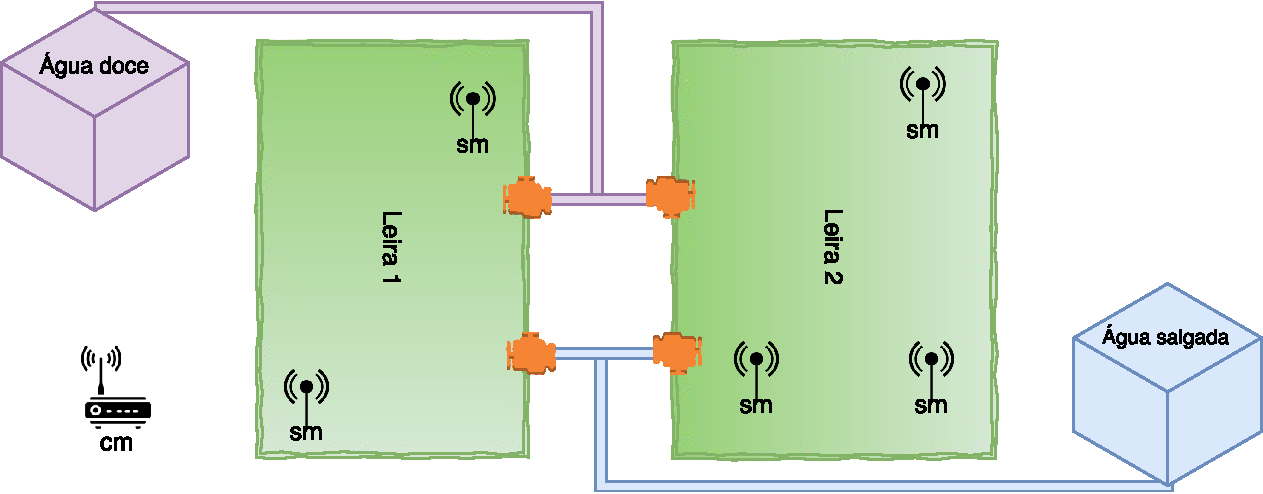
\includegraphics[scale=0.55]{esquemas/leiras-comm-geral.pdf}
	\caption{Ilustração da distribuição dos módulos em leiras para produção de salicornia }
	\label{leira}
\end{figure}


Tal como ilustrado na figura \ref{leira}, pretende-se que sejam colocados módulos com sensores (\acl{SM}) distribuídos estrategicamente por cada leira. Cada um desses módulos irá comunicar com um módulo central (\acl{CM}), originando uma topologia de rede em estrela.  Por sua vez, cada um destes módulos central irá comunicar diretamente com a servidor que possibilitará que os dados sejam tratados e disponibilizados para visualização ao cliente. Pressupõe-se portanto que este ultimo módulo tenha necessariamente ligação à rede de modo a conseguir consumir a API REST por HTTP desenvolvida para o efeito. 


falar mais sobre as plataformas 



\newpage
\section{Componentes}

No contexto desta dissertação é necessário reter dois conceitos principais, são eles: 

\begin{itemize}
	\item \textbf{\textit{\acl{SM}}:} consiste num módulo responsável pela aquisição de dados provenientes dos mais diversos tipos de sensores.
	
	
	\item \textbf{\textit{\acl{CM}}:} consiste num módulo responsável pela receção dos dados/estados do \acl{SM} e respetivo envio para a \textit{cloud}.  
	
\end{itemize}


O cenário da figura \ref{esquema1} ilustra três \acl{SM} que comunicam com um \acl{CM}. Cada um desses \acl{SM} possui um conjunto especifico de sensores e comunica com \acl{CM} através de um determinado modulo de comunicação. Posteriormente, o \acl{CM} possui um determinado protocolo de comunicação que permite a utilização de uma API REST criada para o efeito. 




\begin{figure}[h]
	\centering
	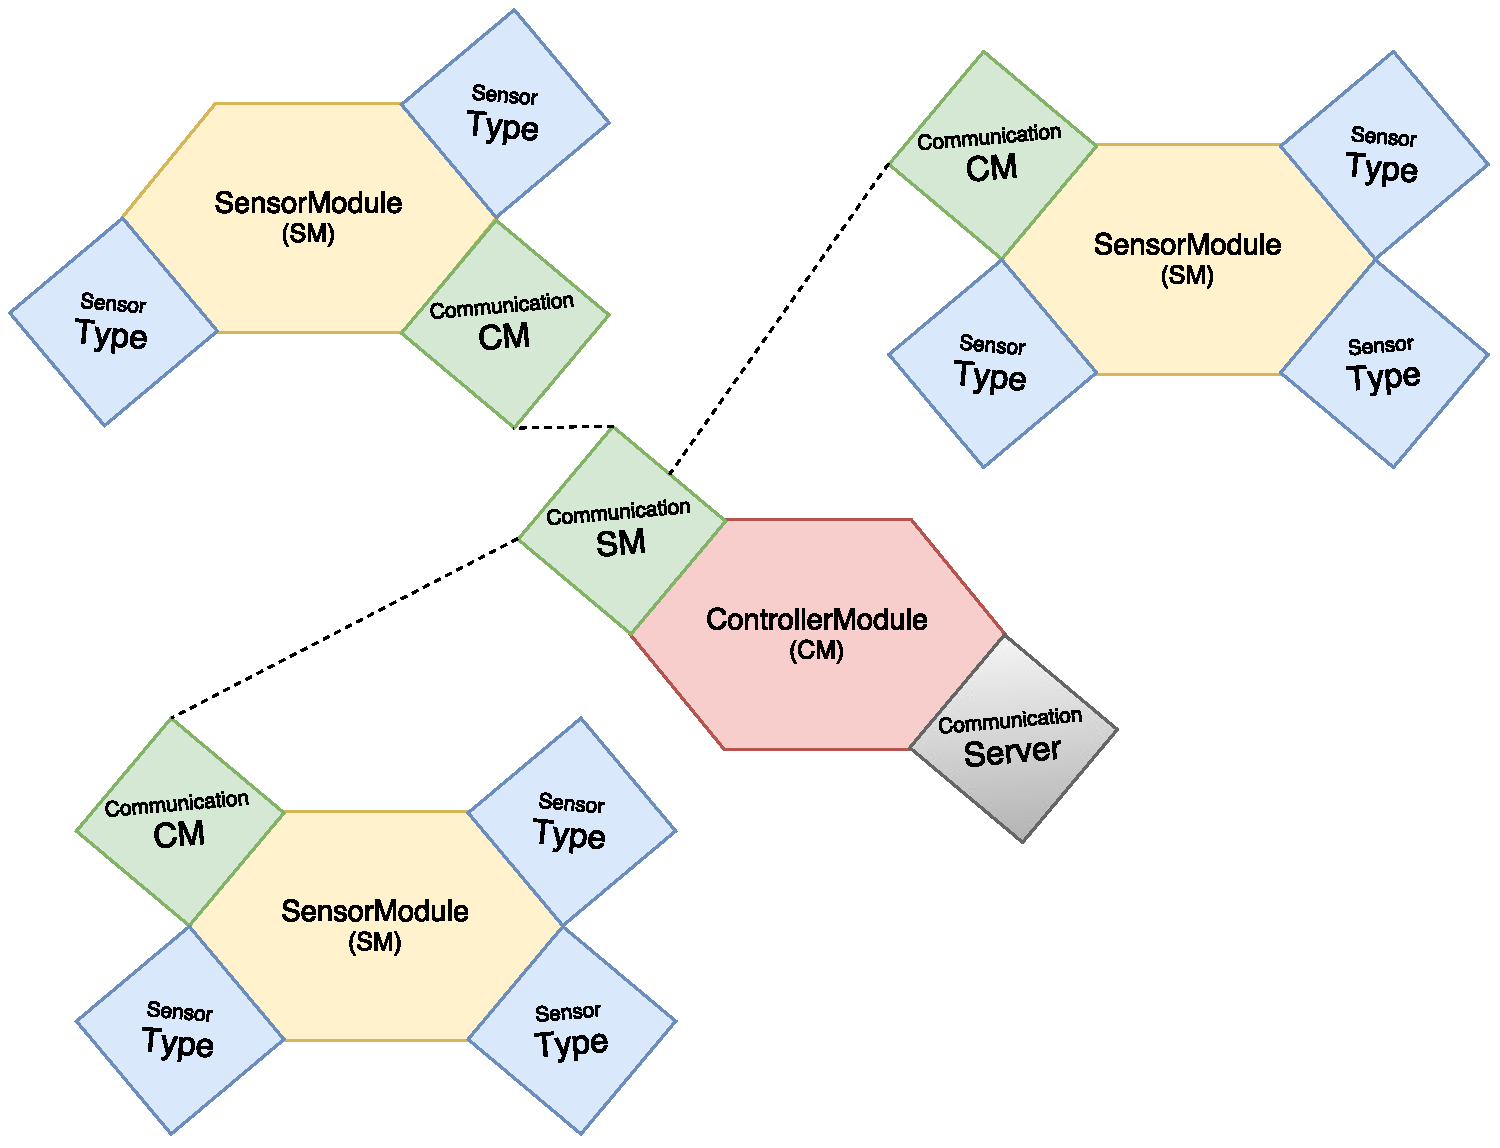
\includegraphics[width=\linewidth]{esquemas/general-electronic-modules.pdf}
	\caption{Esquema de componentes da comunicação de três \ac{SM} com um \ac{CM}}
	\label{esquema1}
\end{figure}


Seguidamente serão especificados todos os detalhes de cada modulo, uma vez que serão considerados na modelação de todo o sistema. 



\newpage
\subsection{\acl{SM}}



Um \acl{SM} consiste num microcontrolador responsável pela aquisição de dados provenientes dos mais diversos tipos de sensores. Cada \acl{SM} terá que utilizar um determinado módulo de comunicação de modo a possibilitar a comunicação com um módulo central. Para além disso, pretende-se que o sensor module possa ter controlo sobre si, ou seja, inteligência própria. 

Prentede-se que este módulo seja identificado por um determinado nome, possua uma bateria que permita a sua mobilidade, um ou vários modulos de comunicação que permita comunicar com um módulo centrar, uma memoria e um módulo \ac{GPS} que permita aceder à sua localização. Para além disso, um \acl{SM} terá que possuir um ou vários sensores.  





\subsection{\acl{CM}}



\acl{CM} consiste num microcontrolador responsável pela receção dos dados preveniente dos \acl{SM}. Pretende-se que este módulo envie informações para os \acl{SM} quando requisitados pelo utilizador. O principal objetivo deste módulo consiste em receber a informação proveniente dos \ac{SM} e respectivo envio para um servidor em \textit{cloud}. 

Pretende-se que este módulo seja identificado por um determinado nome, tenho um  módulo de comunicação que possibilite o envio de dados para o servidor e um campo que nos permita definir o tempo de receção desses dados. Para alem disso, pretende-se que exista um módulo de \ac{GPS} que permita localizar o \acl{CM} em caso de robo.
 





\newpage

%\section{Design funcional}






\section{Análise de requisitos}

Durante o desenvolvimento um software pressupõe-se que os seus intervenientes sigam determinadas metodologia para o seu programa possa revolucionar a vida de um grupo em especifico ou até mesmo da sociedade. 


O ciclo de vida do desenvolvimento de um software, também conhecido como \ac{SDLC}, é composto genericamente por quatro fase principais: concepção, projeto, criação e a implementação. Antes do \ac{SDLC}, o processo de desenvolvimento do software foi tomado como atividade informal sem regras e padrões formais. Isso poderá levar a vários problemas, tais como o atraso no desenvolvimento, aumento de custos e baixa qualidade do software criado. 

O ciclo de vida do desenvolvimento de um software dá o padrão necessário e as etapas para o desenvolvimento de um software com qualidade. Existem enumeros modelos e visões para o ciclo de vida de desenvolvimento, o que a seguir descrevo foi considerado por Munish Kaur \cite{Saini2014}. A figura \ref{sdlcartic} mostra as várias etapas que compõe este modelos e que seguidamente são descritas. 


\begin{figure}[!htb]
	\centering
	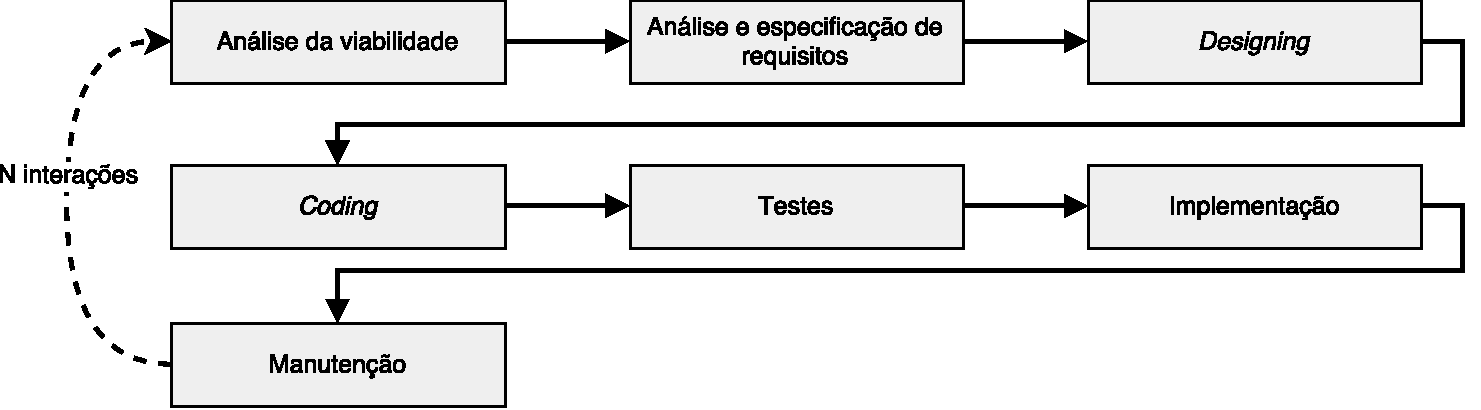
\includegraphics[scale=0.6]{esquemas/desenvolvimentoSW.pdf}
	\caption[Fase de desenvolvimento de um software ]{Fase de desenvolvimento de um software (Adaptado de \cite{Saini2014})}
	\label{sdlcartic}
\end{figure}




\begin{itemize}
	\item \textbf{Análise de viabilidade}: nesta fase é analisada a viabilidade do projeto, sendo analisados dados de entrada e saida, processamento necessário, análise de custos e planeamento do projeto. Nesta fase é incluida a viabilidade técnica em termos de software, hardware e pessoas qualificadas. 
	
	\item \textbf{Analise e especificação de requisitos}: nesta fase são recolhidos e analisados os requisitos necessário para a elaboração do \textit{software}. Pretende-se que no final desta fase sejam conhecidos os vários requisitos do software e seja também criado um documento que os especifique. 
	
	\item  \textbf{\textit{Designing}}: consiste na tradução dos requisitos especificado na fase anterior para a estrutura lógica.Pretende-se que seja elaborado um documento de especificação do \textit{design}. 
	
	
	\item  \textbf{\textit{Coding}}: o programação real é elaborada nesta fase. O documento de \textit{design} é traduzido para o código-fonte numa determinada linguagem de forma a que possa ser executado. 
	
	\item \textbf{Testes}: o código-fonte gerado na fase anterior é testado usando vários cenários de testes. São usadas várias técnicas de teste para avaliar a correção e validação do \textit{software}. 
	
	\item  \textbf{Implementação}: o software desenvolvido é implementado para que possa ser disponbilizado ao utilizador para uso real. Pretende-se que o utilizado do sistema possa reportar erros ou problemas quando encontrados. 
	
	\item  \textbf{Manutenção}: o software poderá sofrer alterações que possam solucionar problemas que tenham ocorrido. Esta fase é responsável pela pós-implementação e manutenção do software para o seu bom funcionamento.
	
\end{itemize}




%http://www.sersc.org/journals/IJSEIA/vol8_no3_2014/38.pdf




A forma como um software realiza as tarefas para as quais foi desenvolvido determina a eficiência de execução do mesmo\cite{Requirementsengineering}. O levantamento de requisitos é umas das fases essenciais no processo de desenvolvimento de um determinado sistema, que nos leva a entender o que o cliente deseja ou acredita precisar levando-nos à criação dos processos de negócio do sistema. 


Seguidamente são apresentados os requisitos funcionais e não funcionais do sistema. 




\subsection{Requisitos funcionais}


Os requisitos funcionais descrevem os critérios que devem ser usados para avaliar as funções especificas ou os comportamentos de um determinado sistema. Seguidamente são apresentados os requisitos funcionais propostos pelo cliente no contexto deste projeto para as duas plataformas disponíveis: web (dashboard) e mobile. 


\textbf{Aplicação mobile (dashboard)}


\begin{itemize}
	\item A interface do sistema deve permitir que o utilizador, seja ele qual for, entre ou faça \textit{login} no sistema. 
	
	\item A interface do sistema deve permitir que o utilizador, seja ele qual for, saia ou faça \textit{logout} no sistema.
	
	\item O dashboard deverá permitir que qualquer utilizador possa recuperar a sua chave de acesso ao sistema.
	
	\item O sistema deve permitir que qualquer utilizador se possa registar no sistema, embora tenha que estar obrigatoriamente associado a uma empresa.
	
	\item O utilizador comum só terá acesso à sua área reserva após a validação por parte da empresa.   
	
	\item O dashboard deverá permitir ao administrador a adição de novas empresas e a gestão de todos os utilizadores. 
	
	\item O sistema deve permitir que qualquer utilizador possa adicionar, editar ou remover: 
	\begin{itemize}
		\item Tipos de sensores
		
		\item Tipos de comunicação
		
		\item Controller modules com as suas caracteristicas
		
		\item Tipo de comunicação a um controller modules que permite a comunicação como servidor 
		
		\item Sensor modules a um determinado controller modules e as suas características 
		
		\item Um ou vários tipos de comunicação de um Sensor moduel
		
		\item Um ou vários sensores a um sensor module em que cada sensor é de um determinado tipo 
		
	\end{itemize}
	
	\item Visualizar graficamente os dados de cada sensor para um determinado \ac{SM}. 
	
	
	\item Visualizar em modo tabular (dataset) os dados de cada sensor para um determinado \ac{SM}. 
	
	\item Em cada uma das visualizações anteriormente descritas, pretende-se que seja possível uma filtragem por data
	
	
	\item O sistema permitirá a exportação dos dados de um determinado \ac{SM} em formato \ac{CSV}. 
	
	\item O sistema deverá disponibilizar uma API que...  
	
	\item Consultar a documentação da API 
	
	\item Consultar o token de autenticação da API 
	
	
	
	\item Alterar configurações do utilizador 
	
	
	
\end{itemize}


\textbf{Aplicação mobile}



\begin{itemize}
	\item A interface da aplicação mobile deve permitir que o utilizador, seja ele qual for, entre ou faça \textit{login} no sistema. 
	
	\item A interface da aplicação mobile deve permitir que o utilizador, seja ele qual for, saia ou faça \textit{logout} no sistema.
	
	
	\item Visualizar graficamente os dados de cada sensor para um determinado \ac{SM}. 
	
	\item Receber alarmes quando um determinado valor lido está fora do estipulado.
	
	
\end{itemize}



\subsection{Requisitos não funcionais}


Requisitos não funcionais são todos os requisitos da aplicação relacionados com
performance, escalabilidade, segurança, disponibilidade e usabilidade. Estes não são
necessariamente pedidos pelo cliente. 


\begin{itemize}
	\item O sistema deverá executar em qualquer plataforma, tanto web como mobile. 
	
	
	\item A base de dados deve ser protegida para acesso apenas a utilizadores autorizados. 
		
	
	\item O sistema deverá disponibilizar uma API para que possam ser criados novos produtos com base neste 
	
	\item Deverá ser usada, na medida do possível, tecnologias sem qualquer custo para o cliente (\textit{opensource}). 
	
	\item Pretende-se que o sistema possa ser adaptado a qualquer outro contexto. 
	

	
	
\end{itemize}



\section{Modelação}

A conceção de uma arquitetura envolve o estudo e modelacao de compontes que sao necessários para a elaboracao da mesma, bem como a analise dos casos de uso, modelos de dados e diagramas de fluxos, entre outros, para melhor entender como emparelhar a estrutura pretendida. Na secção será... %% rever... .................. 



\subsection{Entidades envolventes}




No contexto do sistema descrito existem três entidades distintas que são importantes descrever: 

\begin{itemize}
	
	\item \textbf{General user}: este poderá registar-se e associando-se a uma determinada empresa registada no sistema. Após a validação por parte da empresa, este utilizador poderá aceder à sua área reservada através das dashboard ou da aplicação mobile. 
	
	\item \textbf{Company user}: utilizador que gere todos os general users que se possam associar à sua empresa. Deste modo, este utilizador poderá validar os general users que a si se associam ou eliminá-los.  
	
	\item \textbf{Administrador}: vulgarmente denominado por Admin. Pretende-se que apenas exista uma único administrador. Genericamente este utilizador tem a possibilidade de poder adicionar novas empresas ao sistema, isto é, criar novas utilizador com permissões especificas. 
	
\end{itemize}




\subsection{Casos de uso}


Nas figuras \ref{usedash} e \ref{useMobile} encontram-se representados os esquemas dos casos de uso da \textit{dashboard} (denominada por saliDashboard) e da aplicação \textit{mobile} (denominada por saliMobile), respectivamente.
Seguidamente serão descritos cada um dos casos de uso para as duas plataformas. De notar que todos os casos de uso na aplicação mobile também se encontram disponíveis através da dashboard. 


\begin{figure}[!htb]
	\centering
	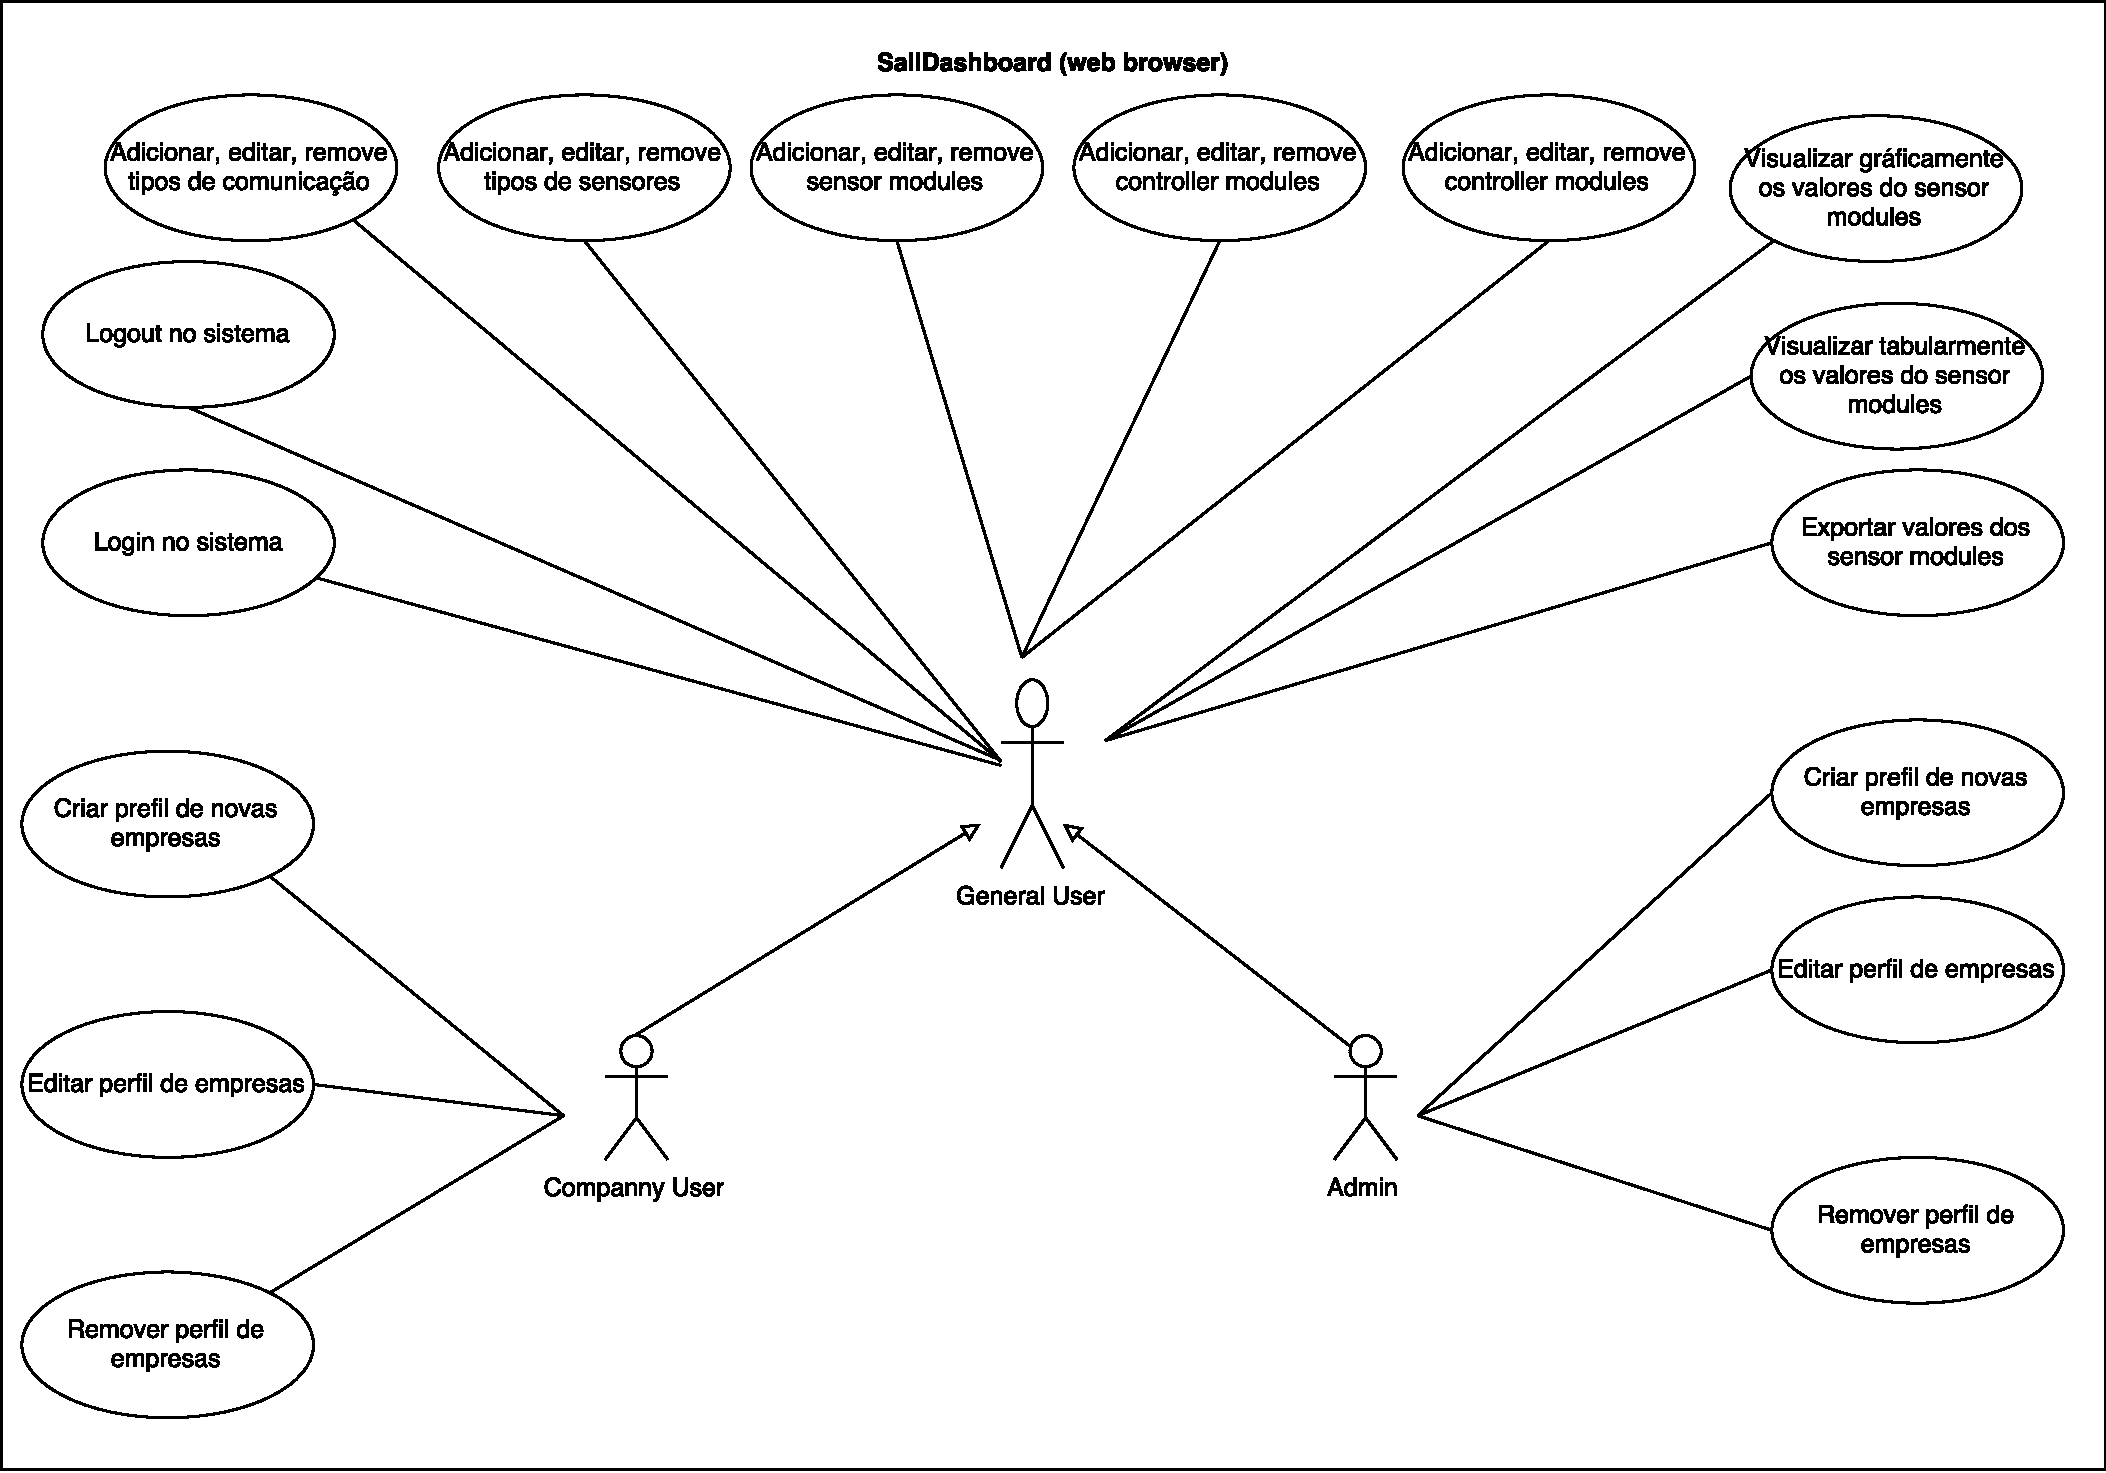
\includegraphics[width=\linewidth]{esquemas/use-case-web.pdf}
	\caption{Casos de uso para a aplicação web (dashboard) }
	\label{usedash}
\end{figure}


\newpage
\begin{figure}[!htb]
	\centering
	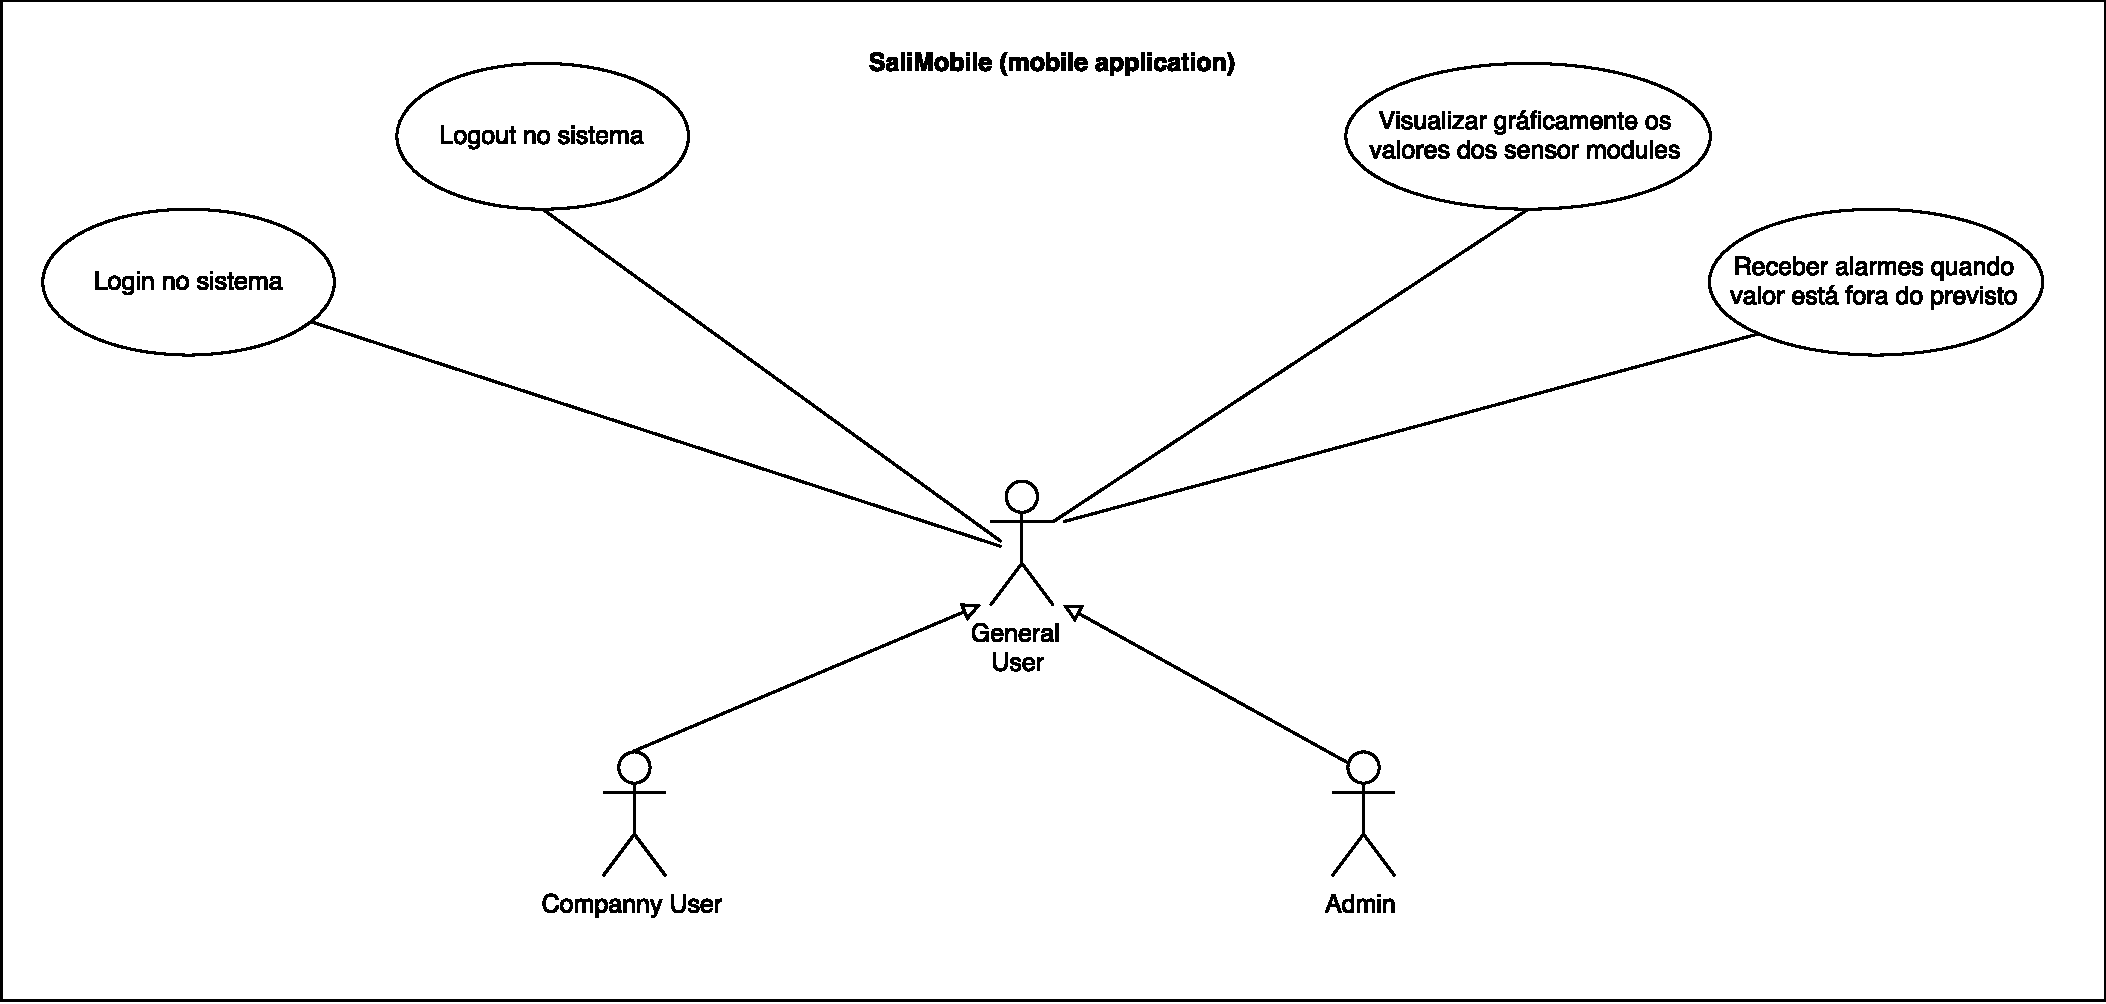
\includegraphics[width=\linewidth]{esquemas/use-case-mobile.pdf}
	\caption{Casos de uso para a aplicação mobile}
	\label{useMobile}
\end{figure}





\begin{itemize}
	\item \textbf{Login no sistema}: qualquer utilizador (general user, company user ou admin) poderá aceder ao sistema tendo para ir que possuir uma conta registada e validada no caso do user general. Após a validação das suas credenciais (username e password) o utilizador poderá aceder à pagina inicial da dashboard e a todo o seu conteúdo. Este caso de uso encontra-se disponível para os dois tipos de plataformas. 
	
	
	\item \textbf{Logout no sistema}: qualquer utilizador (general user, company user ou admin) poderá sair da sistema tendo que para isso tenha que estar obrigatoriamente logado no sistema. Após o logout ser-lhe-á apresentado novamente a página de login. Este caso de uso encontra-se disponível para os dois tipos de plataformas. 
	
	
	\item \textbf{Recuperar password}: qualquer utilizador (general user, company user ou admin) poderá recuperar a sua password de acesso ao sistema, para isso, terá que introduzir o seu email e posteriormente ser-lhe-á envia o acesso que possibilita a redefinição da mesma. 
	
	
	
	\item \textbf{Adicionar, editar, remover tipos de comunicação}: qualquer general user ou company user poderá adicionar, editar ou remover os tipos de comunicação existentes no sistema. Ao  adicionar, o utilizador terá que introduzir um nome, um caminho relevante para o tipo de comunicação e selecionar um icon ilustrativo. No caso da remoção, esta ação apenas é possível caso o tipo de comunicação não se encontre em utilização por nenhum \ac{CM} ou \ac{SM}.  
	
	\item \textbf{Adicionar, editar, remover tipos de sensores}: qualquer general user ou company user poderá adicionar, editar ou remover os tipos de sensores existentes no sistema. Ao  adicionar, o utilizador terá que introduzir um nome que o identifique, uma fonte de dados ou a escala dos dados  e um icon que identifique o sensor. Para além disso, o utilizador terá que escolher uma cor que identifique o tipo de sensor na dashboard. No caso da remoção, esta ação apenas é possível caso o tipo de sensor não se encontre em utilização por nenhum \ac{SM}.   
	 
	
	\item \textbf{Adicionar, editar, remover um controller module}: qualquer \textit{general user} ou \textit{company user} poderá adicionar, editar ou remover um controller module existente no sistema. Neste caso, pressupõe-se que o utilizador possua um micro-controlador com as seguintes características que podem ser adicionadas: determinado nome que o identifique, valor da memória RAM em MB, estado inicial (ativo ou desativo) e um modulo de comunicação que permita comunicar com o servidor web. Estas características são possíveis de alteração. Pretende-se que o controller module possa ser removido tendo \ac{SM} a sí associado, sendo estes também removidos dos sistema. 


	\item \textbf{Adicionar, editar, remover um sensor modules}: qualquer \textit{general user} ou \textit{company user} poderá adicionar, editar ou remover um sensor module existente no sistema. Pressupõe-se o utilizador possui um determinado micro-controlador com um ou mais sensores. Para adicionar o \ac{SM} à plataforma o utilizador terá que atribuir um nome que o identifique, definir qual o seu estado inicial (ativo ou desativo), escolher que tipos de comunicação possam estar presentes e definir o intervalo de tempo para o qual pretende receber os dados lidos pelos sensores. Para além disso, permite associar ao \ac{SM} os sensores presentes e definir o valor máximo e minimos para o qual são gerados alarmes e respectivas mensagens informativas. Todos os dados são possíveis de edição.  
	

	
	\item \textbf{Receber notificações (gerar alarmes)}: sempre que um valor lido por um determinado sensor sai fora do limite imposto (valor máximo e valor mínimo) é gerado um alarme para o utilizador de modo a que este possa intervir. Este caso de uso encontra-se disponível para os dois tipos de plataformas. 
	
	
	\item \textbf{Visualizar gráficamente os dados lidos pelos sensores}: 
	
	
	Este caso de uso encontra-se disponível para os dois tipos de plataformas. 
	
	
	\item Visualizar tabularmente os dados lidos pelos sensor
	
	\item \textbf{Exportar dados lidos por um sensor module}: qualquer \textit{general user} ou \textit{company user} poderá exportar os dados lido pelos sensores para um ficheiro do tipo \ac{CSV} para uma data especificada.
	
	\item \textbf{Visualizar a localização dos módulos (SM/CM)}: qualquer \textit{general user} ou \textit{company user} ao aceder à dashboard ser-lhe-à apresentado um mapa para cada \ac{CM} com a sua localização e dos seus respetivos \ac{SM}. 
	
	
	\item \textbf{Consultar a documentação da API}: qualquer \textit{general user} ou \textit{company user} poderá aceder à dashboard para consultar a documentação da API existente. 
		
	\item \textbf{Consultar token de autenticação}: qualquer \textit{general user} ou \textit{company user} poderá aceder ao token de autenticação para utilização da API. 
	

	
	\item \textbf{Validar general user}: qualquer company user tem a possibilidade de validar os general users que a si se associam. Sempre um novo general user é registado no sistema o comapny user é notificado via email. Posteriormente, caso o general user seja validado este também receberá um email de confirmação.  
	
	\item \textbf{Remove general user}: qualquer company user tem a possibilidade de remove os general users que a si estão associados. 
	
	
	\item \textbf{Remover sensor modules e controller modules }: o admin do sistema tem a possibilidade de remover os sensores modules e/ou controller modules existentes no sistema. 
	
	
	\item \textbf{Visualizar todos os sensor modules e controller modules}: o admim do sistema tem a possibilidade de visualizar todos os sensores modules e controller modules existentes no sistema de modo a alertar os clientes em caso de anomalias. 
	
	
	\item \textbf{Criar um novo company user}: o admim tem a possibilidade de adicionar novos company user ao sistema, sendo para isso necessário 
	
	\item \textbf{Remover um company user}: o admim tem a possibilidade de remover qualquer company user registado no sistema.
	
	
\end{itemize}







De acordo com a figura \ref{useMobile} , é possível descrever os seguintes casos de uso: 






\newpage
\subsection{Modelo de dados}

Depois da análise de requisitos desenhou-se um modelo de dados que permitisse modelar todo o sistema descrito, obtendo-se assim o seguinte esquema relacional apresentado na figura \ref{esquemarelacional}.





\begin{figure}[!htb]
	\centering
	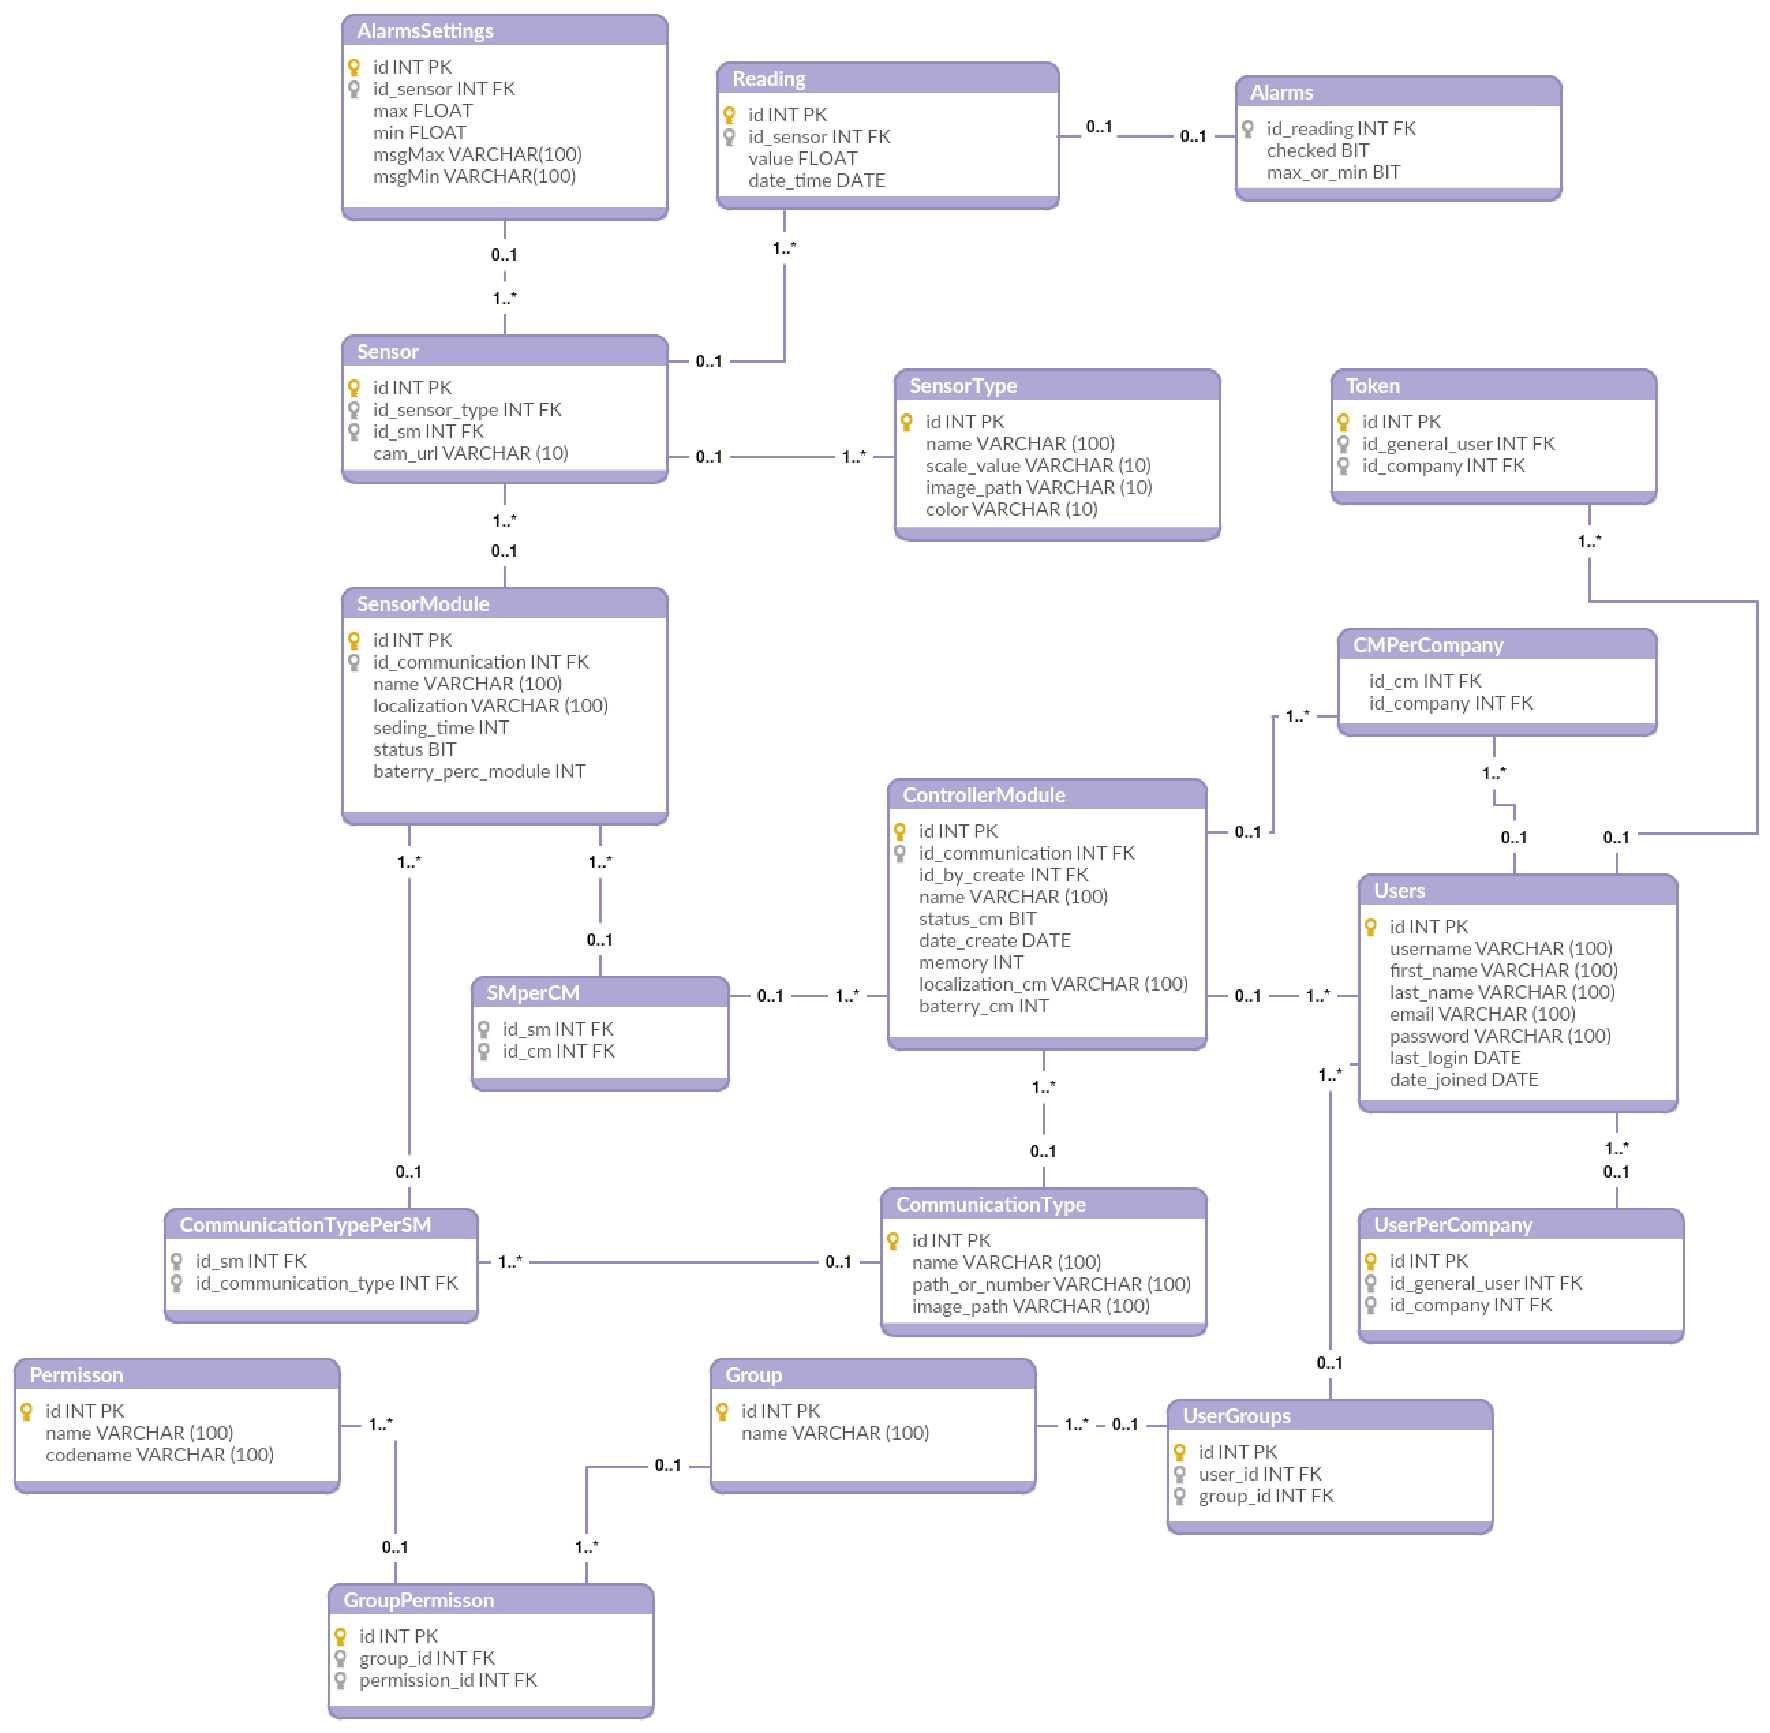
\includegraphics[width=\linewidth]{esquemas/database_tese.pdf}
	\caption{Esquema relacional da estrutura da base de dados}
	\label{esquemarelacional}
\end{figure}


Nas tabelas \ref{tabeladb1} e \ref{tabeladb2} são descritos descritos cada uma das tabelas de dados existentes neste sistema, evidenciando as chaves primária e estrangeiras de cada uma. 



\newpage
\begin{landscape}
	
\begin{table}[]
	\centering

	
	\begin{tabular}{|
			>{\columncolor[HTML]{EFEFEF}}l |l|l|l|}
		\hline
		\textbf{Nome da tabela} & \cellcolor[HTML]{EFEFEF}\textbf{Chave primária (\acs{PK})} & \cellcolor[HTML]{EFEFEF}\textbf{Chave estrangeira (\acs{FK})} & \cellcolor[HTML]{EFEFEF}\textbf{Descrição} \\ \hline
		\textbf{User} & id (auto-incrementado) & N/A & \begin{tabular}[c]{@{}l@{}}Identifica cada um dos \\ utilizadores inseridos no sistema\end{tabular} \\ \hline
		\textbf{Token} & \begin{tabular}[c]{@{}l@{}}authtoken\_token\_pkey\\ (character varying(40))\end{tabular} & user\_id & \begin{tabular}[c]{@{}l@{}}Possui o token de autenticação \\ do utilizador para a API\end{tabular} \\ \hline
		\textbf{Group} & id (auto-incrementado) & N/A & \begin{tabular}[c]{@{}l@{}}Possui todos os grupos \\ existentes: general user,\\ company user e admin\end{tabular} \\ \hline
		\textbf{UserGroups} & id (auto-incrementado) & user\_id group\_id & \begin{tabular}[c]{@{}l@{}}Permite associar um \\ utilizador a um\\  determinado grupo\end{tabular} \\ \hline
		\textbf{Permisson} & id (auto-incrementado) & N/A & \begin{tabular}[c]{@{}l@{}}Possui todas as permissões \\ existentes (escrita, leitura,\\  delete...)\end{tabular} \\ \hline
		\textbf{GroupPermisson} & id (auto-incrementado) & group\_id permission\_id & \begin{tabular}[c]{@{}l@{}}Associa a cada groupo \\ determinadas permissões\end{tabular} \\ \hline
		\textbf{UserPerCompany} & id (auto-incrementado) & company\_id general\_user\_id & \begin{tabular}[c]{@{}l@{}}Associa cada general user\\  a um company user\end{tabular} \\ \hline
		\textbf{CommunicationType} & id (auto-incrementado) & N/A & \begin{tabular}[c]{@{}l@{}}Identifica cada um dos tipos \\ de comunicação inseridos \\ no sistema\end{tabular} \\ \hline
		\textbf{ControllerModule} & id (auto-incrementado) & N/A & \begin{tabular}[c]{@{}l@{}}Identifica cada um dos \\ controller module \\ inseridos no sistema\end{tabular} \\ \hline
	\end{tabular}
	\caption{My caption}
	\label{tabeladb1}
\end{table}


\newpage




\begin{table}[]
	\centering

	
	\begin{tabular}{|
			>{\columncolor[HTML]{EFEFEF}}l |l|l|l|}
		\hline
		\multicolumn{1}{|c|}{\cellcolor[HTML]{EFEFEF}\textbf{Nome da tabela}} & \multicolumn{1}{c|}{\cellcolor[HTML]{EFEFEF}\textbf{Chave primária (PK)}} & \multicolumn{1}{c|}{\cellcolor[HTML]{EFEFEF}\textbf{Chave estrangeira (FK)}} & \multicolumn{1}{c|}{\cellcolor[HTML]{EFEFEF}\textbf{Descrição}} \\ \hline
		\textbf{CMPerCompany} & id (auto-incrementado) & \begin{tabular}[c]{@{}l@{}}cm\_id\\ company\_id\end{tabular} & \begin{tabular}[c]{@{}l@{}}Associa todos os controller module\\  a um determinado company user\end{tabular} \\ \hline
		\textbf{SensorModule} & id (auto-incrementado) & N/A & \begin{tabular}[c]{@{}l@{}}Identifica cada um dos sensor \\ module inseridos no sistema\end{tabular} \\ \hline
		\textbf{SMperCM} & id (auto-incrementado) & \begin{tabular}[c]{@{}l@{}}cm\_id\\ sm\_id\end{tabular} & \begin{tabular}[c]{@{}l@{}}Associa os sensor modules a \\ um determinado controller module\end{tabular} \\ \hline
		\textbf{CommunicationTypePerSM} & id (auto-incrementado) & \begin{tabular}[c]{@{}l@{}}communication\_type\_id\\ \\ sm\_id\end{tabular} & \begin{tabular}[c]{@{}l@{}}Permite associar a um sensor \\ module um ou várias tipos \\ de comunicação\end{tabular} \\ \hline
		\textbf{SensorType} & id (auto-incrementado) & N/A & \begin{tabular}[c]{@{}l@{}}Identifica cada um dos tipos \\ de sensores inseridos no sistema\end{tabular} \\ \hline
		\textbf{Sensor} & id (auto-incrementado) & \begin{tabular}[c]{@{}l@{}}sensor\_type\_id\\ sm\_id\end{tabular} & \begin{tabular}[c]{@{}l@{}}Permite identificar um \\ determinado sensor\end{tabular} \\ \hline
		\textbf{AlarmsSettings} & id (auto-incrementado) & sensor\_id & \begin{tabular}[c]{@{}l@{}}Permite guardar as configurações \\ para um determinado sensor\\ (max,min…)\end{tabular} \\ \hline
		\textbf{Reading} & id (auto-incrementado) & sensor\_id & \begin{tabular}[c]{@{}l@{}}Permite guardar as leituras de \\ um determinado sensor\end{tabular} \\ \hline
		\textbf{Alarms} & id (auto-incrementado) & reading\_id & \begin{tabular}[c]{@{}l@{}}Armazena os alarmes \\ que são gerados\end{tabular} \\ \hline
	\end{tabular}
	\caption{My caption}
	\label{tabeladb2}
\end{table}

\end{landscape}



\newpage
\section{Arquitetura lógica}

Nesta secção é apresentada uma arquitetura lógica do sistema, indicando as camadas que este deverá conter, especificando quais as relações de dependência que estas possuem entre si. Seguidamente, é explicado como implementar esta lógica com os respetivos componentes físicos. 


Normalmente este tipo de arquitetura é composto por três camadas com intenções diferentes: camada de apresentação, camada de lógica de negócio e camada de acesso a dados. Pretende-se que com a descrição desta arquitetura seja facilitada a manutenção, a portabilidade e a
escalabilidade, fatores importantes quando queremos partilhar funcionalidades e informação entre aplicações de diferentes tipos.




\begin{figure}[!htb]
	\centering
	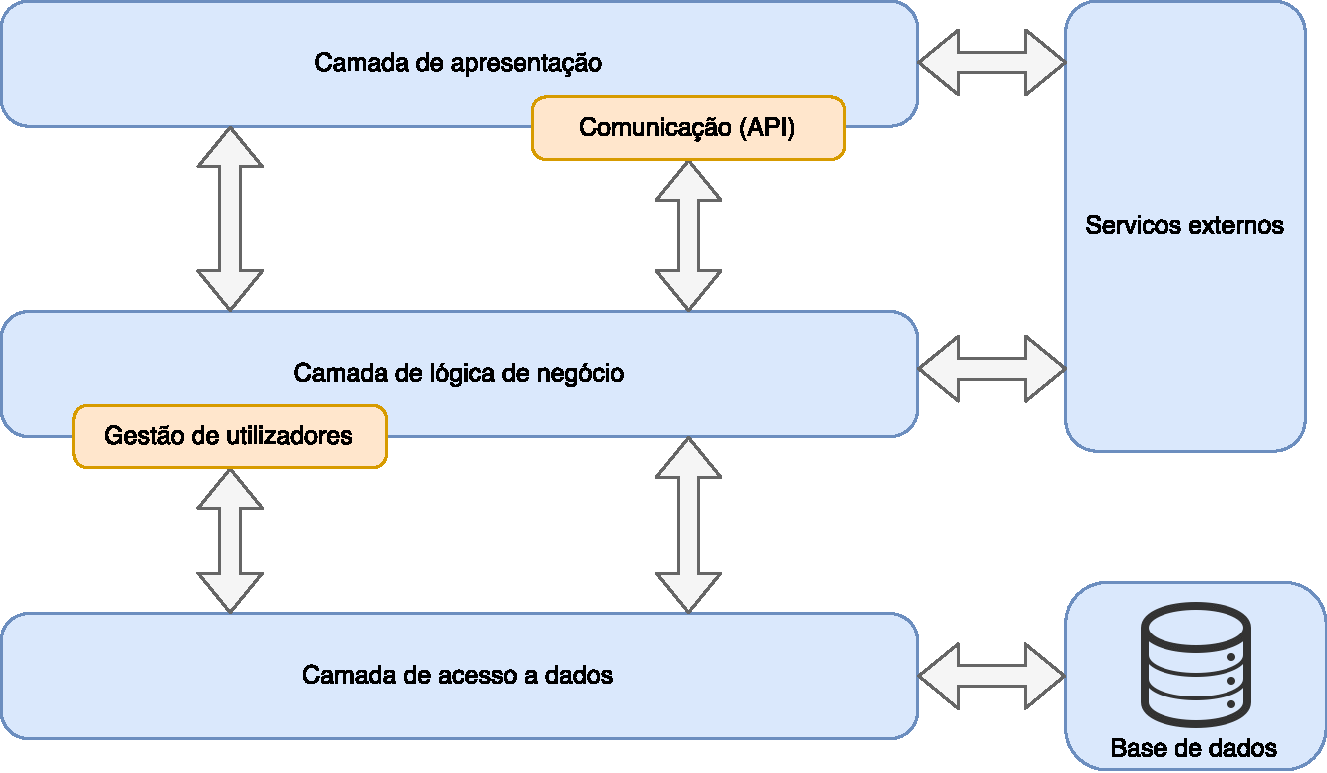
\includegraphics[scale = 0.6]{esquemas/arquitetura-logica.pdf}
	\caption{Arquitetura lógica}
	\label{opencvlogo}
\end{figure}



\subsection{Camada de apresentação}


A camada de apresentação é responsável pela comunicação entre os utilizadores e a aplicação, sendo ela web ou mobile, exibindo informações aos utilizadores, abrangendo uma interface que permite solicitações ao sistema. Esta camada tem uma relação de dependência com a camada de lógica de negócio e tira partido do acesso a serviços de informação externos, que fornecem diversas funcionalidades. 


A interface do utilizador foi desenvolvida em  \ac{HTML} e \acs{CSS}, fazendo uso de jQuery e Javascript.



\begin{itemize}
	\item \ac{HTML} é a linguagem padrão usada para estruturar e apresentar conteúdos na web. Neste caso, foi utilizado HTML5, a quinta versão do \ac{HTML}.
	\item \ac{CSS} é uma linguagem usada para descrever a apresentação de conteúdo escrito em uma marcação Como HTML.
	
	\item \ac{JS} é a linguagem de programação para páginas da web.
	\item \textbf{JQuery}: JQuery é uma biblioteca Javascript que simplifica a programação Javascript
\end{itemize}









\subsection{Camada de lógica de negócio}



verificar se valor se encontra lido se encontra dentro dos settings e gerar alarme 


\subsection{Camada de acesso a dados}


Nesta camada deverão estar presentes as funcionalidades de criação, edição, remoção ou simples de visualização dos dados, sendo responsável pelas operações de persistência e consulta de dados solicitadas pela camada de lógica de negócio.




\newpage
\section{Arquitetura física}


Enquanto que a arquitetura lógica se concentra nos diferentes níveis de abstração do sistema a arquitetura física foca-se na estrutura de alto nível.  
Seguidamente são apresentados todos os componentes físicos, tanto  a nível de software com de hardware, que são fundamentais para ter um maior perceção do real funcionamento de todo o sistema. 
A figura \ref{fisicablocos} representa genericamente os blocos principais do sistema proposto que seguidamente serão descritos. 


\begin{figure}[h]
	\centering
	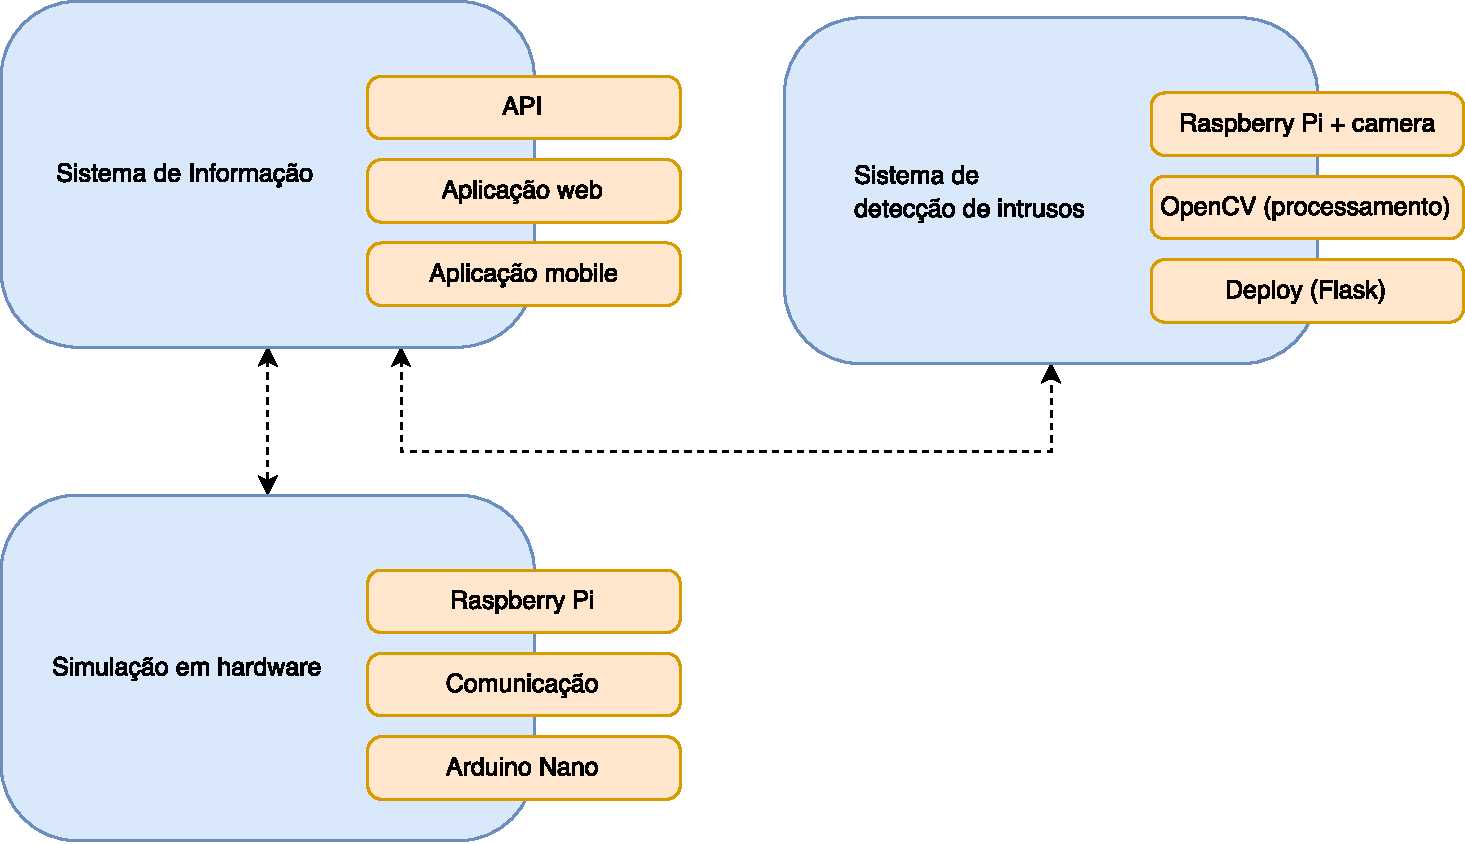
\includegraphics[scale=0.45]{esquemas/esquema-blocos.pdf}
	\caption{Arquitetura física (blocos)}
	\label{fisicablocos}
\end{figure}


  
\subsection{Sistema de informação}


Segundo Laudon et al. \cite{Laudon1998}  um sistema de informação define-se como sendo uma inter-relação de múltiplos componente podendo estes ser equipamentos, telecomunicações, software, bases de dados e outras tecnologias de transformação de informação usadas para recolha, processamento, armazenamento e distribuição de informação que possibilita a tomada de decisões e controlo para uma determinada organização, ou até mesmo para a sociedade em geral, de modo a torná-la mais acessível e útil.

Dada a elevada complexidade de um sistema de informação, é possivel identificar algumas funcionalidade comuns aos diversos sistema, são eles \cite{Turban1996}: 

\begin{itemize}
	\item \textbf{Recolha de dados}: sequência de tarefas que permitem a adição de novos dados ao sistema
	\item \textbf{Organização e armazenamento de dados}: é imprescindível uma boa organização na estrutura de dados possibilitando uma fácil e rápida localização.
	\item \textbf{Processamento de dados}: qualquer funcinalidade que permita a produção de resultados mais úteis do que os dados em bruto. 
	 
	\item \textbf{Distribuição de informação}: após o processamento de dados é fundamental a distribuição destes a quem precise deles.
	
	\item \textbf{Utilização da informação}: por si só, a informação não tem qualquer valor, a sua utilização em contexto adequado permite a extração de determinadas conclusões para que possam ser tomadas decisões.
	
\end{itemize}



A figura \ref{arquiteturasi} ilustra a arquitetura do sistema de informação incluindo especificamente a base de dados, \ac{API}, \textit{dashboard} e respetiva implementação do sistema. 


\begin{figure}[h]
	\centering
	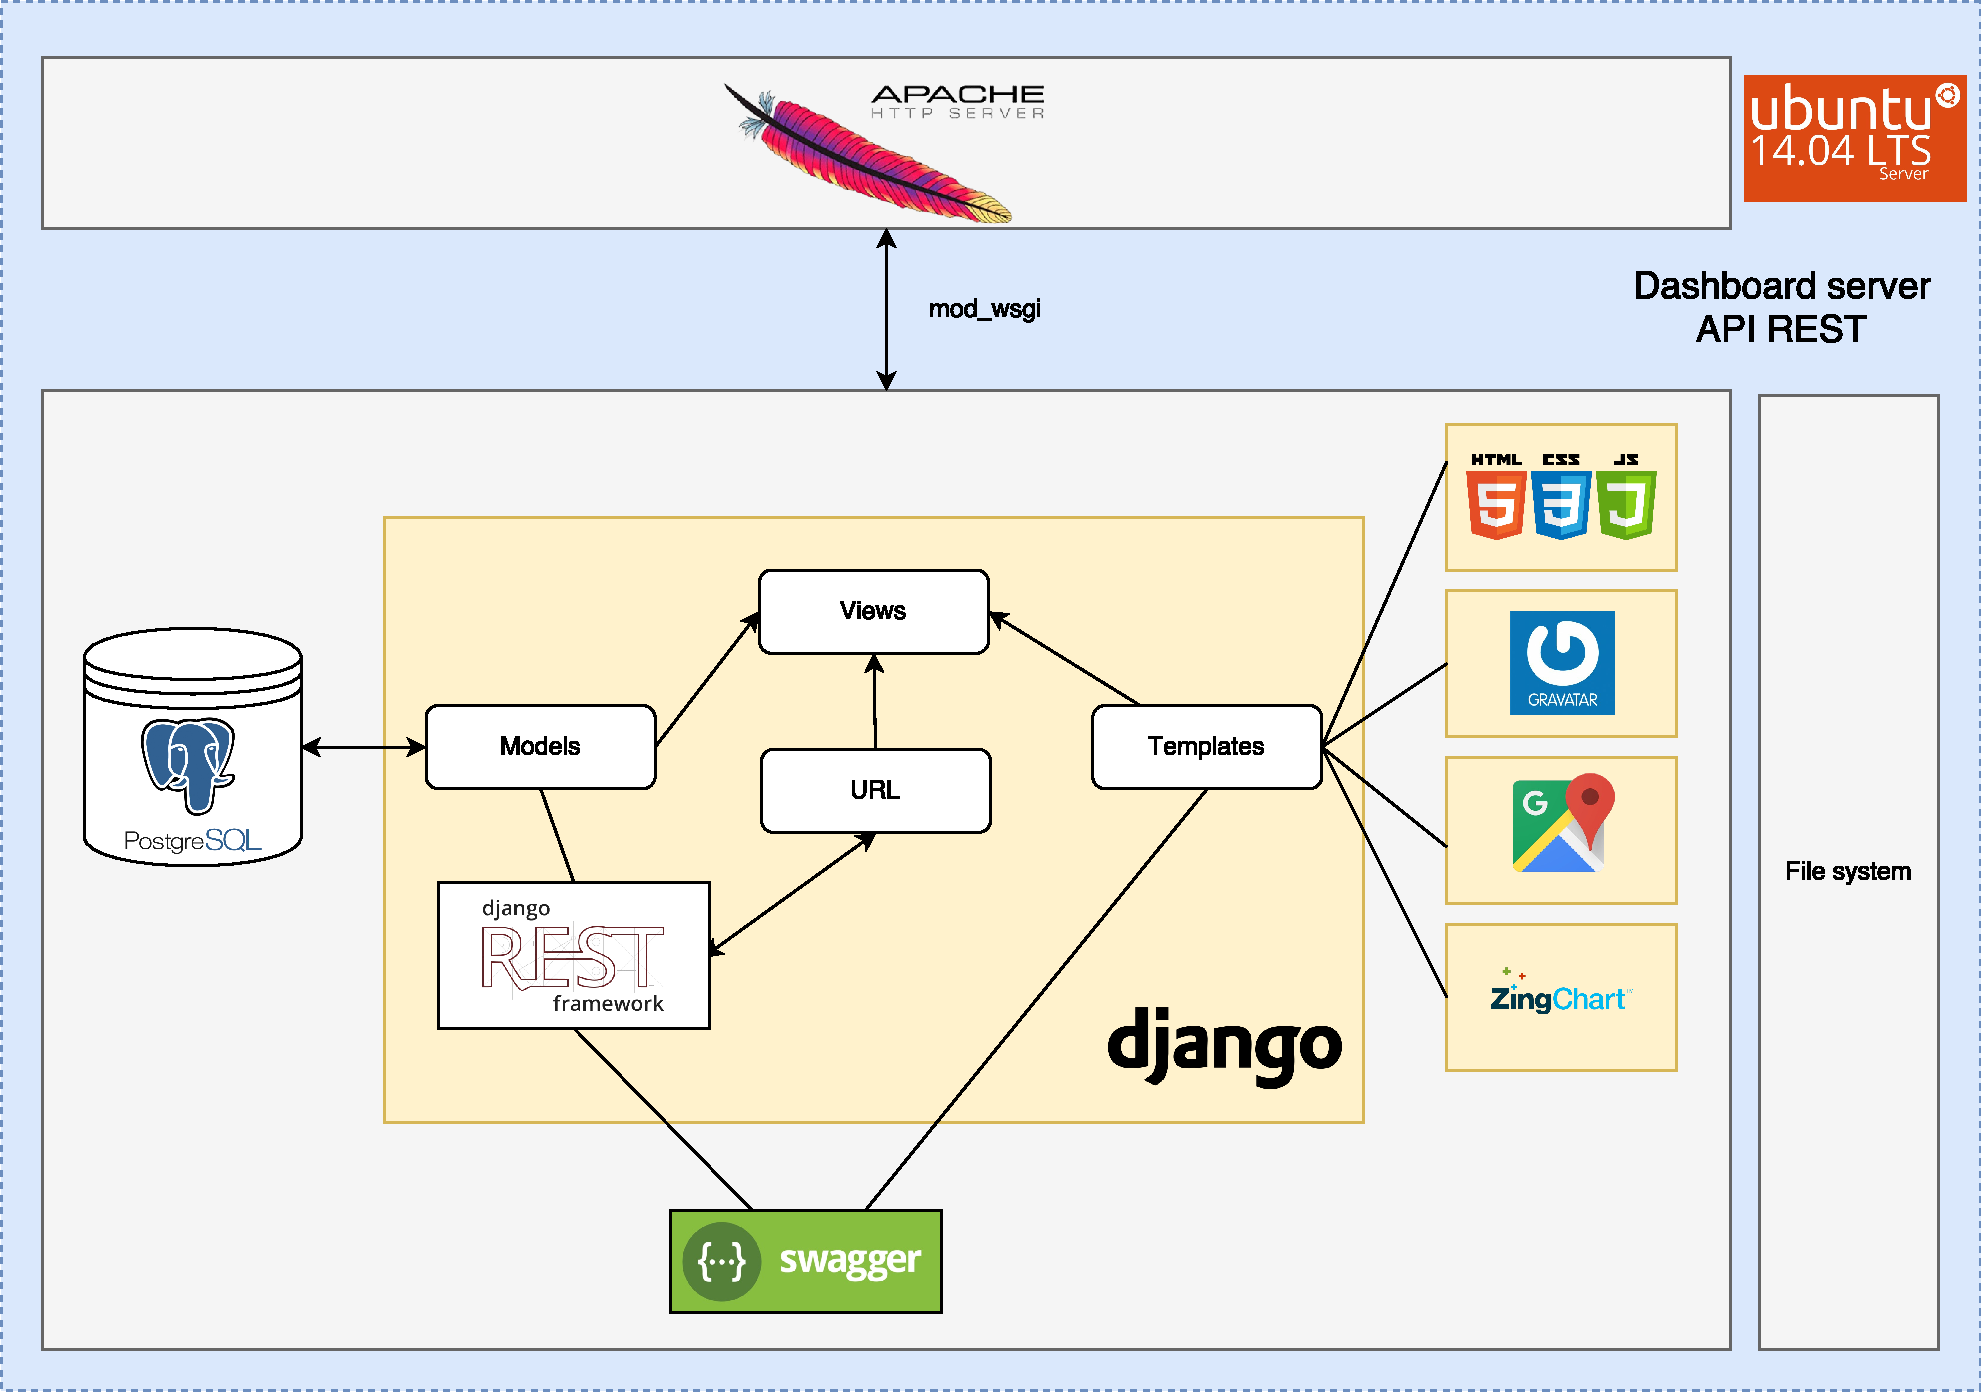
\includegraphics[width=\linewidth]{esquemas/fisica-si.pdf}
	\caption{Arquitetura do sistema de informação (dashboard e API)}
	\label{arquiteturasi}
\end{figure}


\subsubsection{Aplicação web}

A aplicação web é um componente essencial, enquadrando-se na camada de lógica de negócio como também na camada de apresentação, permitindo a interação por parte do utilizador (\textit{frontend}) como também no processamento lógico (\textit{backend}).   

Tal como vimos na secção do estado de arte, a tecnologia para o desenvolvimento web recaiu sobre a \textit{framework} Django, mais precisamente na versão 1.11 para python 2.7, sendo que como \ac{IDE} foi utilizada a verão 2016.3.3 do PyCharm.

Dada a facilidade com que a framework django tem em manipular view e templates, optou-se que tanto o desenvolvimento frontend da aplicação web como obviamente backend seja desenvolvido em Django. Para além disso, optou-se por criar uma API RESt que permitisse a manipulação dos dados existentes na base de dados, sendo esta também desenvolvida paralelamente com a aplicação web. Seguidamente será explicada a sua arquitetura.   

Uma das coisas mais interessantes no Django é sem dúvidas a existência de \ac{ORM}. Consiste numa técnica de desenvolvimento que permite modelar os dados através de classes em Python. Através dela, é possível gerar tabelas na base de dados e manipulá-las sem a necessidade de interagir diretamente com \ac{SQL} (embora também seja possível). Existiu necessidade de criar um script em \ac{SQL} que verifica os valores lido pelos sensores gerandam ou não um alarmes. Caso o valor lido esteja fora dos valores previsto então é gerado um alarme e o utilizador será notificado, no capitulo seguinte será descrita a sua implementação. 

A escolha do \ac{SGBD} recaiu sobre o PostgreSQL, mais concretamente na versão xxx. Como ferramenta gráfica para administração deste \ac{SGBD} foi utilizado o PgAdmin III\footnote{www.pgadmin.org/} na versão 1.22. Este software gráfico tem inúmeras funcionalidades desde a possibilidade de ligação a base de dados remotas até à adição, edição, remoção e  consultas em tabelas. Esta ferramenta é \textit{opensource} e encontra-se disponível para Windows e UNIX.


No que diz respeito à camada de apresentação na plataforma web foram utilizadas as seguintes bibliotecas/frameworks: 

\begin{itemize}
	\item \textbf{\ac{HTML}+\ac{CSS}+\ac{JS}}: o ponto de partida para a criação da interface web assentou no template denominado por AdminLTE sendo este baseado em Bootstrap 3\footnote{http://getbootstrap.com/}. Neste template prevalecem as seguintes características:  design responsivo, interface leve e apelativa, existência de múltiplos plugins, compatibilidade entre navegadores entre outros. 
	
	\item \textbf{Gravatar}: serviço que disponibiliza um avatar que esteja associado a endereços de email registado. O Gravatar disponibiliza uma API que pode ser utilizada nas mais diversas linguagens de programação\cite{gravatar}.
	 
	\item \textbf{\ac{API} Google Maps}: consiste num serviço de pesquisa e visualização de mapas e imagens de satélite. É usado na visualização da localização dos diferentes módulos. 
	
	\item \textbf{ZingChart}: biblioteca em \ac{JS} que permite receber dados a apresentá-los em formato gráfico. Esta solução \textit{opensource} disponibiliza mais de 35 tipos e módulos de gráficos. 
\end{itemize}




Dada da facilidade com que o django tem em  com um SGBD, 



Visualização modulos usados 




Base de dados -> fazer ligação com API 














\subsubsection{\acs{API} \acs{REST}}


Os métodos desta API permitiram execuções funções do tipo \ac{REST}. A tecnologia \ac{REST} foi apresentada por Roy Fielding na Universidade de Califórnia no ano de 2000, cujo o titulo da sua dissertação era "Architectural Styles and the Design of Network-based Software Architectures". Roy estudou um conjunto de arquiteturas de software que usam a Web como uma plataforma para computação distribuída\cite{Rodriguez2015}. 

 
 
Esta tecnologia define um conjunto de princípios...   

 
%%%mudar 
Representational State Transfer (REST) define um conjunto de princípios de arquitetura para
sistemas distribuídos, com os quais podemos desenhar serviços web com foco nos recursos de um
sistema, incluindo a forma com os recursos são organizados e transferidos através de HTTP para
vários clientes em diferentes linguagens




Os métodos da API permitem executar as funções REST usando métodos HTTP explicitamentee. Assim, torna-se fundamental perceber estes métodos para ter um melhor conhecimento da API. Como tal, de seguida, são descritos os métodos mais importantes que dão suporte a cada uma das funções REST.


\begin{itemize}
	\item \textbf{GET}: permite efectuar operações de leitura 
	\item \textbf{POST}: permite realizar operações de escrita, permitindo criar novos recursos ao sistema.
	\item \textbf{PUT}: permite criar ou atualizar um novo objecto ao sistema 
	\item \textbf{DELETE}: permite apagar objecto ou recurso ao sistema. 
\end{itemize}







Como vimos na secão X do estado da Arte, a escolha da framework para construção de uma \ac{API} \ac{REST} recaiu sobre o \textit{Django REST framework}



Endpoints 




framework Django REST é um conjunto de ferramentas poderoso e flexível para a construção de APIs Web.




Autenticação


Seguidamente será apresentada como foi criada a documentação desta API. 

\newpage
\subsubsection{Documentação interativa}


Para a geração automática da documentação da API utilizou-se o Swagger. Tal como descrito no site oficial desta framework \cite{SmartBearSoftware2017}, o Swagger é considerada a ferramenta de APIs mais popular e completa de todo o mundo permitindo facilmente o desenvolvimento do ciclo de vida de uma API, desde o design, documentação, testes e também implementação, tendo a grande vantagem de ser opensource. Neste contexto, apenas será utilizada como documentação, de modo a facilitar a sua interpretação da API criada. O swagger possui uma interface apelativa e intuitiva, 
permitindo interagir com a API e permitindo também que os seus utilizadores tenham uma ideia geral de como esta responde aos pedidos para diversos parâmetros e opções. 


\begin{figure}[h]
	\centering
	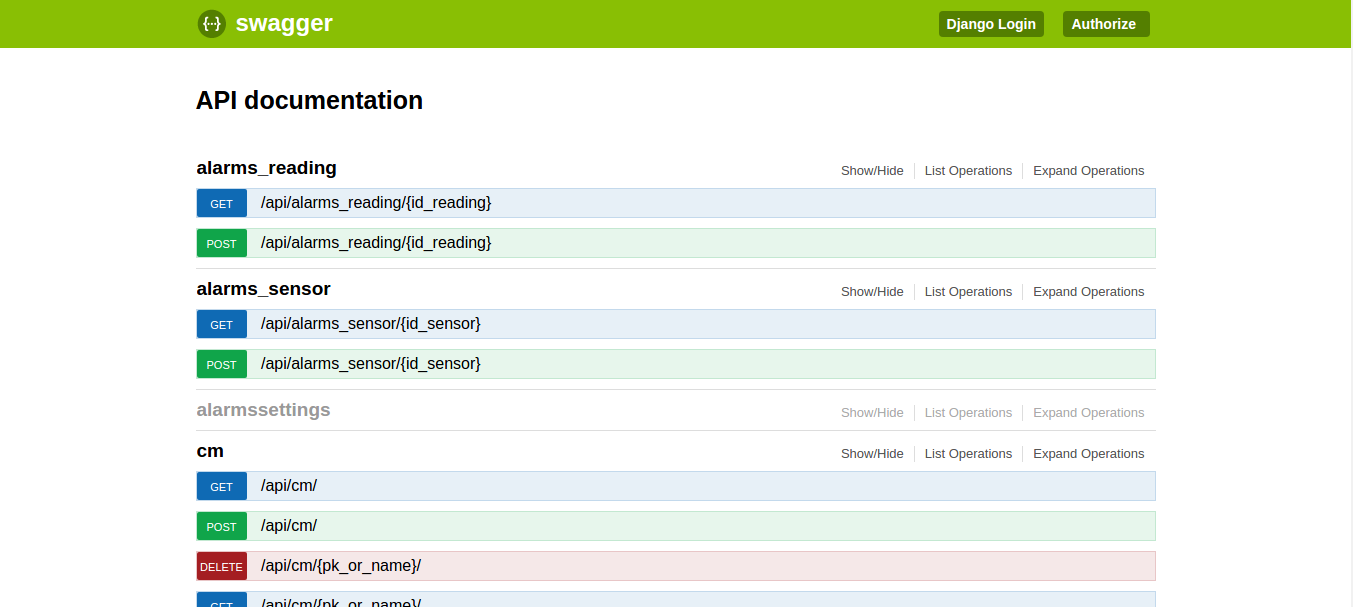
\includegraphics[width=\linewidth]{prints-web/api-doc.png}
	\caption{Arquitetura do sistema de informação (dashboard e API)}
	\label{docapi}
\end{figure}



\subsubsection{Implementação do sistema}

Para implementar (vulgarmente denominada por deployment) o projeto em Django e respetiva API foi-me fornecida uma máquina com um distribuição Linux (Ubuntu 14.04.5) com as seguintes características: 

\begin{itemize}
	\item \ac{CPU}: Intel(R) Xeon(R) CPU E5-2670 v3 @ 2.30GHz
	\item \ac{RAM}: 2 GB
	\item Disco: 10.7 GB
\end{itemize}


Para o processo de \textit{deployment} deste projeto optou-se pela utilização do servidor Apache juntamente com o pacote mod\_wsgi\footnote{https://modwsgi.readthedocs.io/en/develop/}. 
Este pacote fornece uma \ac{WSGI} compatível para o alojamento de aplicações web em Python sob o servidor Apache. 

O Apache é um servidor web opensource mais utilizado em todo o mundo .......

\cite{TheApacheSoftwareFoundation2016}







% implementação falar da incorporação na dashboard e poss





%\section{Documentação automática}

%\subsection{Documentação API}












\subsubsection{Aplicação mobile}


Mockup da aplicação em anexo 

Phonegap + angular js


\begin{figure}[h]
	\centering
	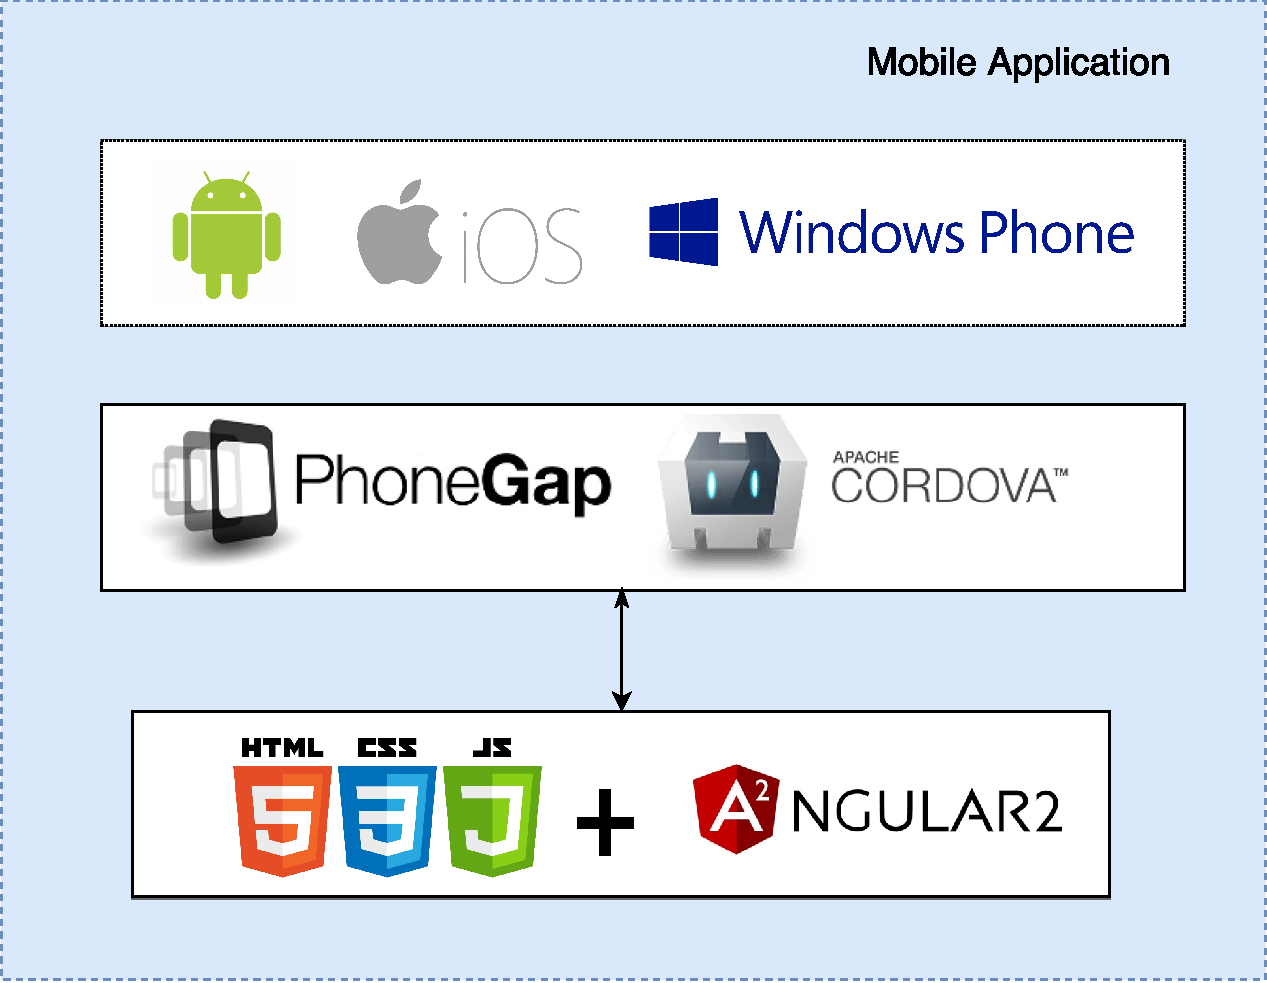
\includegraphics[scale = 0.5]{esquemas/arquitetura-mobile.pdf}
	\caption{Arquitetura do sistema de informação (dashboard e API)}
	\label{arquiteturasi}
\end{figure}



Tal como descrito na secção do estado de arte, para o desenvolvimento mobile optou-se pela utilização de um paradigma multi-plataforma, para tal, escolheu-se o PhoneGap juntamente com o Apache Cordova. 




De modo a facilitar a manipulação em javascript optou-se por utilizar a framework AngularJS. Esta framework opensource mantida pela google desde 20XX 



\newpage
\subsection{Simulação em hardware}


Após a desenvolvimento da API anteriormente descrita, pretendeu-se simular o sistema num contexto real. Para tal, planeou-se encontrar hardware que encaixasse no contexto deste projeto. Foram utilizados dois micro-controladores (Arduino e Raspberry Pi) e alguns sensores. Neste contexto, assume-se que o Arduino é considerado um \ac{SM} que possui um conjunto de sensores enquanto que o Raspberry Pi é um \ac{CM} que recebe os dados provenientes do \ac{SM} enviando-os para o servidor web.  

Seguidamente, são apresentados os sensores utilizados bem como o tipo de comunicação. 
 

\subsubsection{Sensores utilizados}

Nesta secção serão apresentados os sensores utilizados na simulação e as suas principais características. Todos os sensores foram escolhidos tendo em conta o seu enquadramento no projeto e a sua disponibilidade no laboratório. Todos os sensores que se apresentam encontram-se ligados a um Arduino nano. \\

\newpage
\textbf{Temperatura}


Como sensor de temperatura foi utilizado um termístor do tipo \ac{NTC}. Como vimo anteriormente, um termístor é um semicondutor sensível à temperatura i.e. cujo o coeficiente de variação da resistência com a temperatura é negativa, ou seja, quando a temperatura sobe então consequentemente a resistência diminui. 

Na figura \ref{esquema-temp} encontra-se o esquema de ligação deste componente e na tabela \ref{table-temp} as propriedades principais. 


\begin{figure}[h]
	\centering
	\begin{minipage}[b]{0.4\textwidth}
		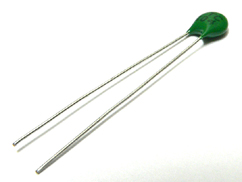
\includegraphics[width=\textwidth]{img/hardware/temperatura.jpg}
		\caption{TTC 104 NTC}
	\end{minipage}
	\hfill
	\begin{minipage}[b]{0.4\textwidth}
		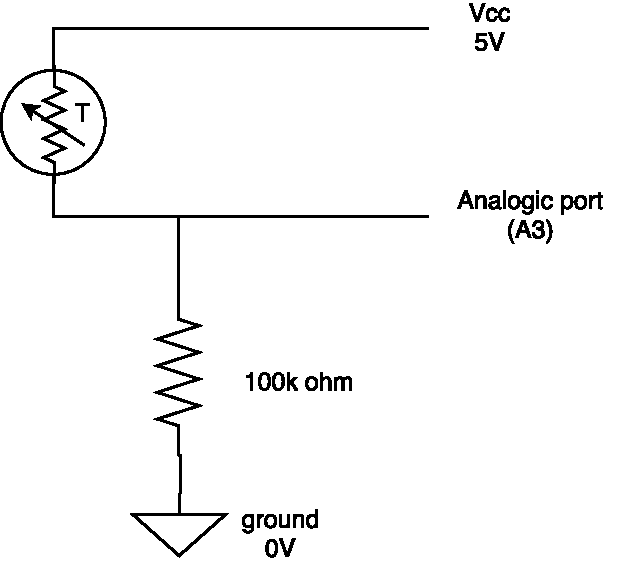
\includegraphics[width=\textwidth]{img/hardware/temp-esquema.pdf}
		\caption{Esquema eletrotécnico da ligação do sensor de temperatura}
		\label{esquema-temp}
	\end{minipage}
\end{figure}



\begin{table}[h]
	\centering
	
	\begin{tabular}{|
			>{\columncolor[HTML]{C0C0C0}}l |l|} \hline
		Dimensão & 5mm \\ \hline
		Resistência & 100K $\Omega$  \\ \hline
		Valor máximo & +125C \\ \hline
		Valor mínimo & -30C \\ \hline
		Nível de confiança & + - 10\% \\ \hline
		Preço & 0.35 \euro/unidade \\ \hline
	\end{tabular}
	\caption[Características do sensor TTC 104]{Características do sensor TTC 104 \cite{temp-dta}}
	\label{table-temp}
\end{table}


\newpage
\textbf{Luminosidade}

Para simular a luminosidade incidente foi utilizado um sensor do tipo foto-resistência. Este sensor, também conhecido como \ac{LDR}, não é mais do que uma resistência variável cujo o seu valor varia conforme a intensidade da luz que incide sobre ele i.e. à medida que a intensidade da luz aumenta, a sua resistência diminui. Este sensor tem múltiplas aplicações, entre as quais se destaca a monitorização solar, indicador da posição do sol (up/down), alarmes anti-roubo, alarme para abertura/fecho de portas entre outras. 

Como vimos na secção X do capitulo do Estado de Arte é um sensor de baixo custo e bastante fácil de utilização. Na figura \ref{lum-esquema} encontra-se o esquema de ligação do componente e na tabela \ref{lum-cara} são apresentadas as principais características do sensor utilizado. 







\begin{figure}[h]
	\centering
	\begin{minipage}[b]{0.4\textwidth}
		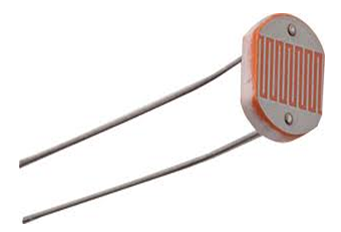
\includegraphics[width=\textwidth]{img/hardware/luminosidade.png}
		\caption{Sensor foto-resistência GL5528}
	\end{minipage}
	\hfill
	\begin{minipage}[b]{0.4\textwidth}
		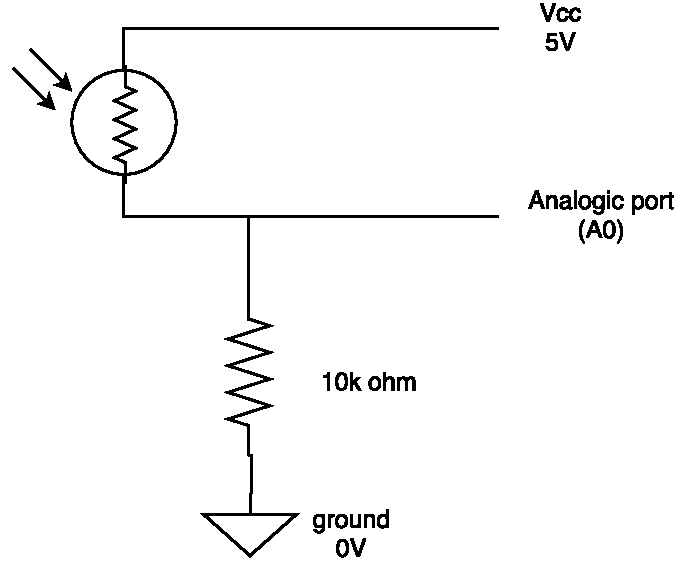
\includegraphics[width=\textwidth]{img/hardware/lumi_esquema.pdf}
		\caption{Esquema eletrotécnico da ligação do sensor de luminosidade}
		\label{lum-esquema}
	\end{minipage}
\end{figure}











\begin{table}[h]
	\centering
	
	\begin{tabular}{|
			>{\columncolor[HTML]{C0C0C0}}l |l|} \hline
		Diâmetro & 5mm \\ \hline
		Tensão máxima & 150VDC \\ \hline
		Potência máxima & 100mW \\ \hline
		Tensão de operação & -30 C a 70 C \\ \hline
		Espectro &540nm \\ \hline
		Comprimento com terminais & 32mm \\ \hline
		Resistência no escuro &1 M (Lux 0) \\ \hline
		Resistência na luz &10-20 Komega (Lux 10) \\ \hline
		Material & Carbono \\ \hline
		Preço & 0.22 \euro/unidade \\ \hline
	\end{tabular}
	\caption[Características do sensor GL5528]{Características do sensor GL5528 \cite{lum-data}}
	\label{lum-cara}
\end{table}


\newpage

\textbf{Sensor de nível líquido}

Este sensor não é mais do que um interruptor que é ativo sempre que um determinado líquido ultrapassa o mesmo. Sempre que algum líquido atingir o pedaço de plástico este irá subir ativando assim o circuito. 
Na figura \ref{esquem-liquido} encontra-se o esquema da ligação deste sensor.




\begin{figure}[h]
	\centering
	\begin{minipage}[b]{0.4\textwidth}
		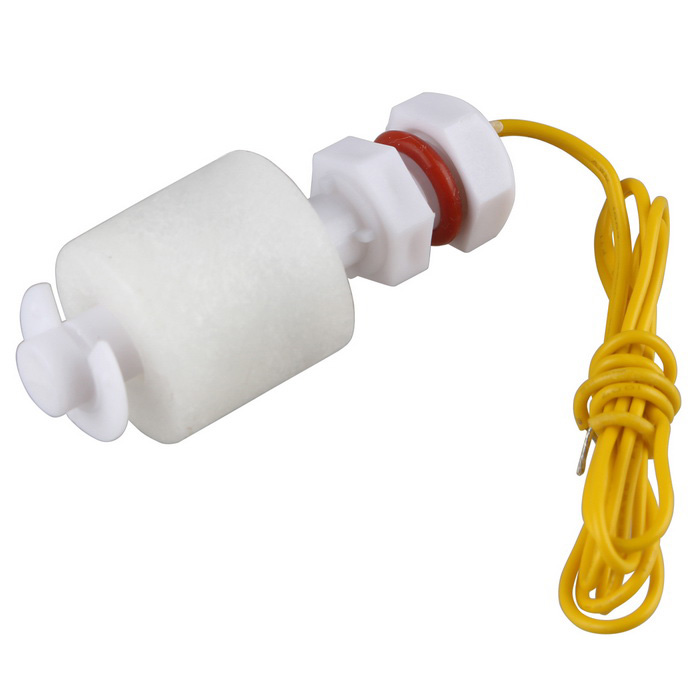
\includegraphics[width=\textwidth]{img/hardware/liquido.JPG}
		\caption{\textit{Water Level Switch Liquid Level Sensor Plastic Ball Float}}
	\end{minipage}
	\hfill
	\begin{minipage}[b]{0.4\textwidth}
		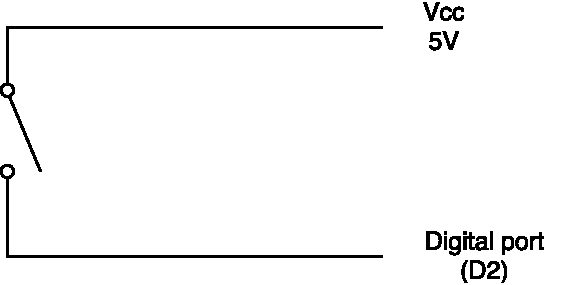
\includegraphics[width=\textwidth]{img/hardware/sw_esquema.pdf}
		\caption{Esquema eletrotécnico da ligação do sensor de nível líquido}
		\label{esquem-liquido}
	\end{minipage}
\end{figure}



\textbf{Simulador de válvula para transferências de águas}

Para a simulação de uma válvula que permitirá as transferência de água doce e salgada foi utilizado um simples \textit{led}. Este possibilita facilmente identificar através da ativação do \textit{led} se a válvula se encontra ativa ou não. 


\begin{figure}[h]
	\centering
	\begin{minipage}[b]{0.4\textwidth}
		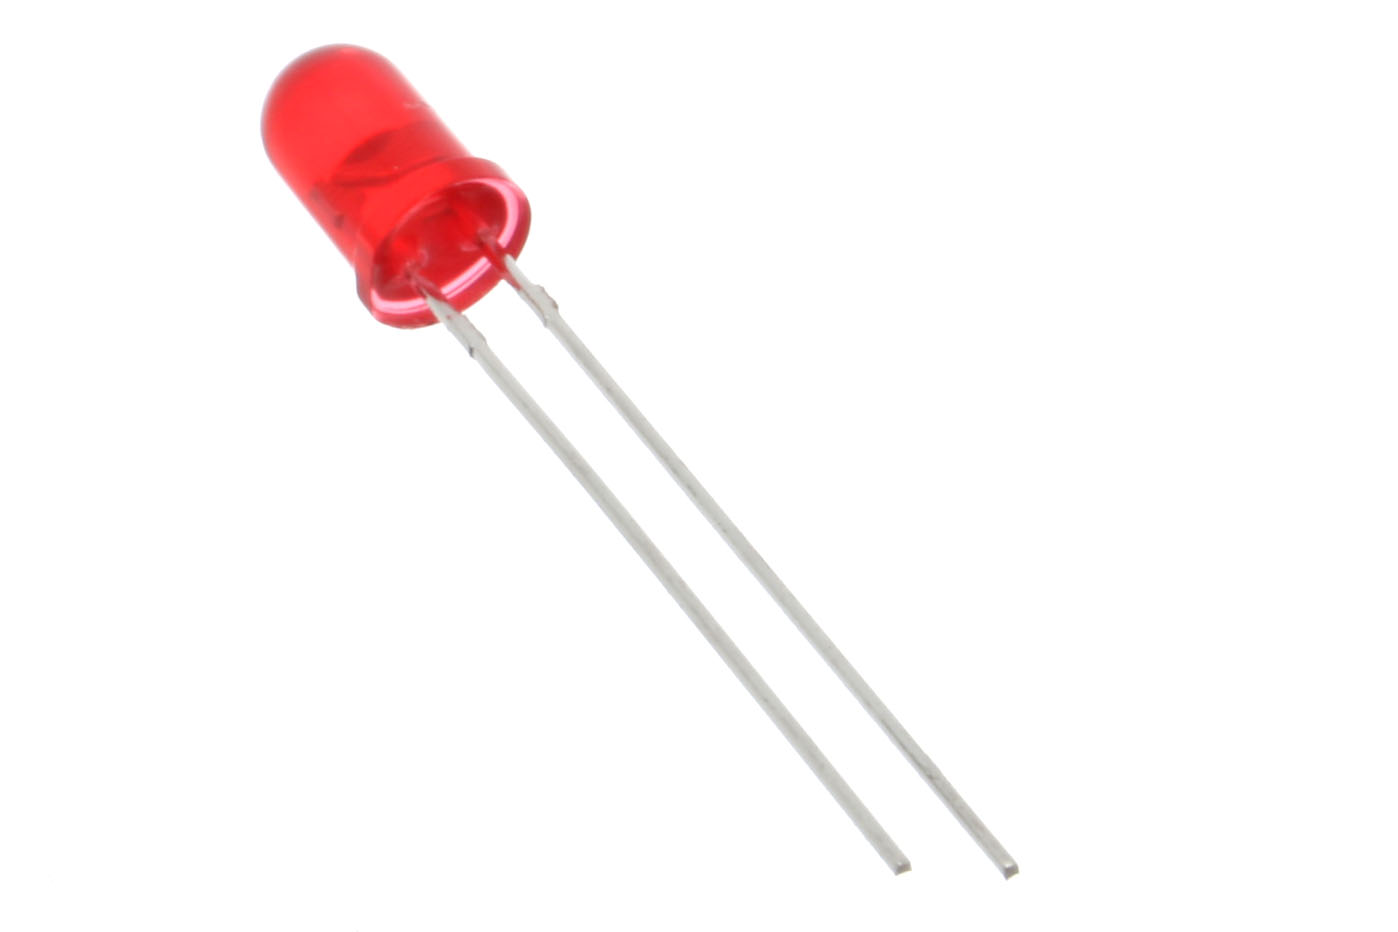
\includegraphics[width=\textwidth]{img/hardware/led.jpg}
		\caption{Led simples.}
	\end{minipage}
	\hfill
	\begin{minipage}[b]{0.4\textwidth}
		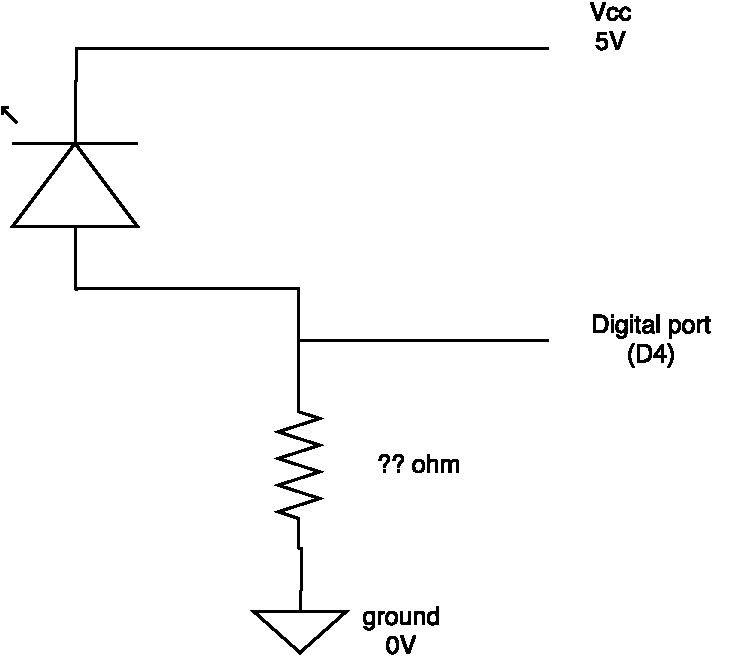
\includegraphics[width=\textwidth]{img/hardware/led_esquema.pdf}
		\caption{Esquema eletrotécnico da ligação do led}
	\end{minipage}
\end{figure}




\newpage
\subsubsection{Comunicação}

Nesta secção, será apresentado o tipo de comunicação para este cenário de simulação. Pretendeu-se que cada um dos módulo ficassem isolados entre si, o que implicou o estudo e respetiva escolha de algumas tecnologias de comunicações sem fio. Neste caso, foram escolhidas as seguintes: 

\begin{itemize}
	\item \textbf{Bluetooth}: utilizado para a comunicação entre o Arduino (\ac{SM}) e o Raspberry Pi 3 (\ac{CM}). No Arduino foi utilizado um módulo Bluetooth HC-06 e no Raspberry Pi 3 foi utilizado o seu próprio módulo interno. 
	\item \textbf{Wifi}: utilizado para a comunicação entre o Raspberry Pi 3 (\ac{CM}) e o servidor. 
\end{itemize}


O esquema da figura \ref{esquemcomm} pretende esquematizar os tipos de comunicação envolvidos nesta simulação para cada um dos componentes. 

\begin{figure}[!htb]
	\centering
	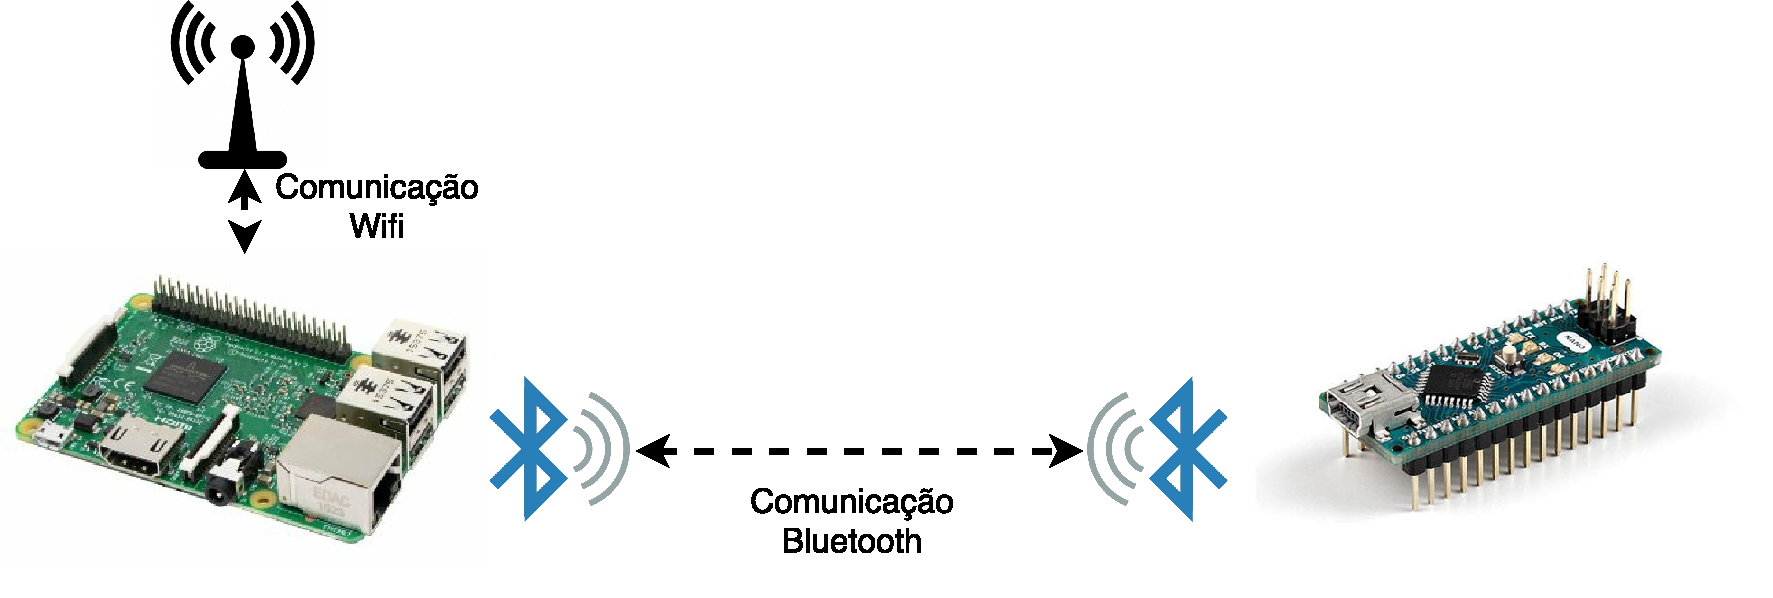
\includegraphics[width=\linewidth]{img/comm-blue/HW-geral.pdf}
	\caption{Arquitetura lógica}
	\label{esquemcomm}
\end{figure}




Módulo bluetooth HC-06



Este módulo bluetooth HC-05 oferece uma forma fácil e barata de comunicação com seu projeto Arduino. Diferente do modelo HC-06, suporta tanto o modo mestre como escravo, além de ter uma fácil configuração.

Em sua placa existe um regulador de tensão e você poderá alimentar com 3.3 a 5v, bem como um LED que indica se o módulo está pareado com outro dispositivo. Possui alcance de até 10m.

é mais uma forma simples e barata de enviar e receber informações remotamente.


\newpage
\begin{figure}[h]
	\centering
	\begin{minipage}[b]{0.4\textwidth}
		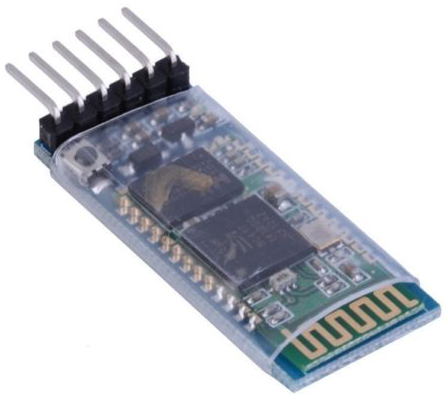
\includegraphics[width=\textwidth]{img/hardware/bluetooth_zs-040.png}
		\caption{Flower one.}
	\end{minipage}
	\hfill
	\begin{minipage}[b]{0.4\textwidth}
		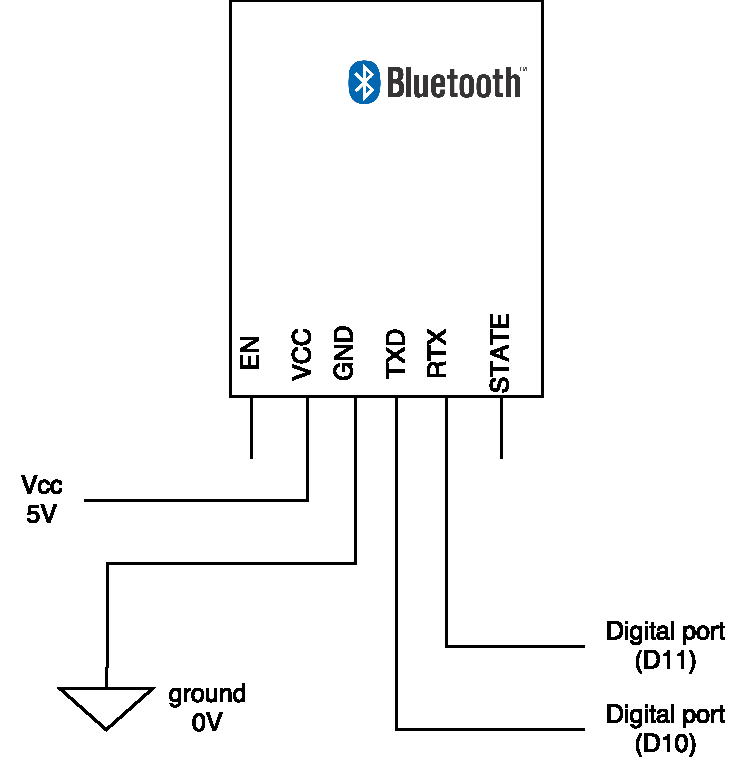
\includegraphics[width=\textwidth]{img/comm-blue/electronic-sensors.pdf}
		\caption{Esquema eletrotécnico da ligação do módulo bluetooth}
	\end{minipage}
\end{figure}



\begin{table}[h]
	\centering
	
	\begin{tabular}{|
			>{\columncolor[HTML]{C0C0C0}}l |l|} \hline
		Diâmetro & 5mm \\ \hline
		
		Protocolo Bluetooth& v2.0+EDR \\ \hline 
		Frequência& 2,4GHz Banda ISM \\ \hline
		Segurança& Autentificação e Encriptação \\ \hline
		Tensão& 3,3v (2,7-4.2v) \\ \hline
		Alcance& 10m \\ \hline
		Dimensões& 26,9 x 13 x 2,2mm \\ \hline
		Peso& 9,6g \\ \hline
		Preço&32\euro /unidade  \\ \hline
	\end{tabular}
	\caption[Características do sensor GL5528]{Características do sensor GL5528 \cite{lum-data}}
	\label{lum-cara}
\end{table}



%http://www.instructables.com/id/Modifying-the-AT-Codes-on-a-HC-05-With-the-Code-ZS/


%http://www.arduinoecia.com.br/2013/03/modulo-bluetooth-jy-mcu-configuracao.html








\newpage

\section{Sistema de deteção de intrusos}


No contexto desta dissertação houve necessidade de implementar um sistema de video-stream que permitisse detetar intrusos, maioritariamente pessoas ou animais de grande porte, que possam invadir as quintas onde se produz salicornia. Esta necessidade prende-se essencialmente com elevado custo do hardware do sistema de monitorização e também de eventuais instrumentos de elevado custo necessários ao cultivo desta espécie (e.g. geradores, maquinas elétricas para poda etc).

Neste capitulo é descrita a tecnologia de processamento de imagem utilizada tal como o algoritmo disponibilizado pela mesma. Apresenta-se a implementação deste mecanismo e os testes necessários. 


\subsection{Biblioteca de processamento de imagem: OpenCV}

O OpenCV, também conhecido por \textit{Open Source Computer Vision Library}, é uma biblioteca de software de visão por computador de código \textit{open source} (figura \ref{opencvlogo}). OpenCV foi construído para fornecer uma infra-estrutura comum para aplicações de visão computacional e para criar o uso da perceção da máquina nos produtos comerciais.

A biblioteca possui mais de 2500 algoritmos otimizados, que inclui um conjunto abrangente de algoritmos clássicos e avançados de visão computacional e algoritmos de \textit{machine learning}. Esses algoritmos podem ser usados para detectar e reconhecer rostos, identificar objetos, classificar ações humanas em vídeos, detetar movimentos numa câmara, seguir um objetos em movimento, produzir nuvens de pontos 3D de câmaras estéreo, entre outros.
OpenCV tem mais de 47 mil pessoas na comunidade de usuários e o número estimado de downloads superior a 7 milhões. A biblioteca é amplamente utilizada em empresas e grupos de pesquisa \cite{Itseez}.

O OpenCV é usado principalmente em aplicações de visão em tempo real. Esta biblioteca tem interfaces nas mais diversas linguagens: C++, C, Python, Java e MATLAB, embora seja nativamente escrito em C. OpenCV tem suporte para Windows, Linux e Mac OS\cite{Itseez}. 

\begin{figure}[!htb]
	\centering
	
\includegraphics[width=0.5\linewidth]{img/vision/opencv_logo.jpg}
	\caption{Logótipo OpenCV}
	\label{opencvlogo}
\end{figure}


\textbf{Conclusoes} 

Desde logo a escolha da tecnologia para processamento de imagem recaiu sobre o opencv não apenas por ser uma biblioteca bastante popular e possuir bastantes algoritmos implementados mas também por eu próprio possuir já algum background e projetos desenvolvidos neste neste contexto.


Pretendeu-se que este processamento fosse implementado em material já adquirido sem necessidade de gastos. Optou-se então por utilizar um \textit{Raspberry Pi} que juntamente com um \textit{Raspberry Pi camera module} (figura \ref{raspicam}) permitirá a aquisição de imagem e servirá também como \textit{controller module} ao sistema de aquisição de dados. 


\begin{figure}[!htb]
	\centering
	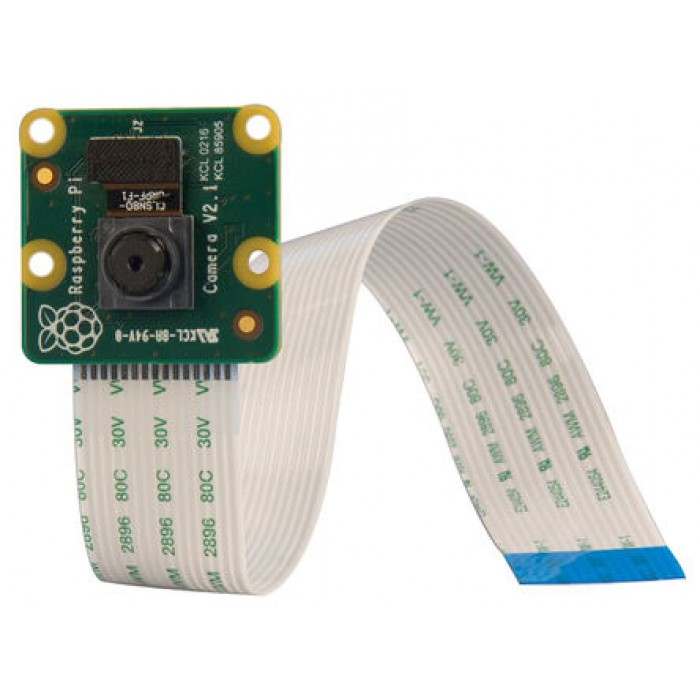
\includegraphics[width=0.3\linewidth]{img/hardware/camera_v2.jpg}
	\caption{Raspberry Pi Camera Board V2 8MP 1080p}
	\label{raspicam}
\end{figure}


Eis algumas das características principais do Raspberry Pi Camera Board V2:

\begin{itemize}
	\item lente de foco fixo on-board
	\item 150 milímetros CSI cabo da câmara incluída
	\item 8 megapixels do sensor com capacidade de resolução nativa de 3.280 imagens estáticas de pixels x 2464
	\item Suporta 1080p30, 720p60 e 640x480p90 vídeo
	\item Tamanho 25 milímetros x 23 milímetros x 9 mm
	\item Peso pouco mais de 3 g
	\item Liga-se à placa de framboesa Pi por meio de um cabo de fita curta (fornecido)
	\item Camera v2 é compatível com a última versão do Raspbian, sistema operacional preferido do Raspberry Pi
\end{itemize}






%%%%%%%%%%%%%%%%%%%%%%%%%%%%%%%%%%%%%%%%%%%%%%%%%%%%%%%%%%

\newpage
\section{Diagrama de componentes}

\begin{figure}[!htb]
	\centering
	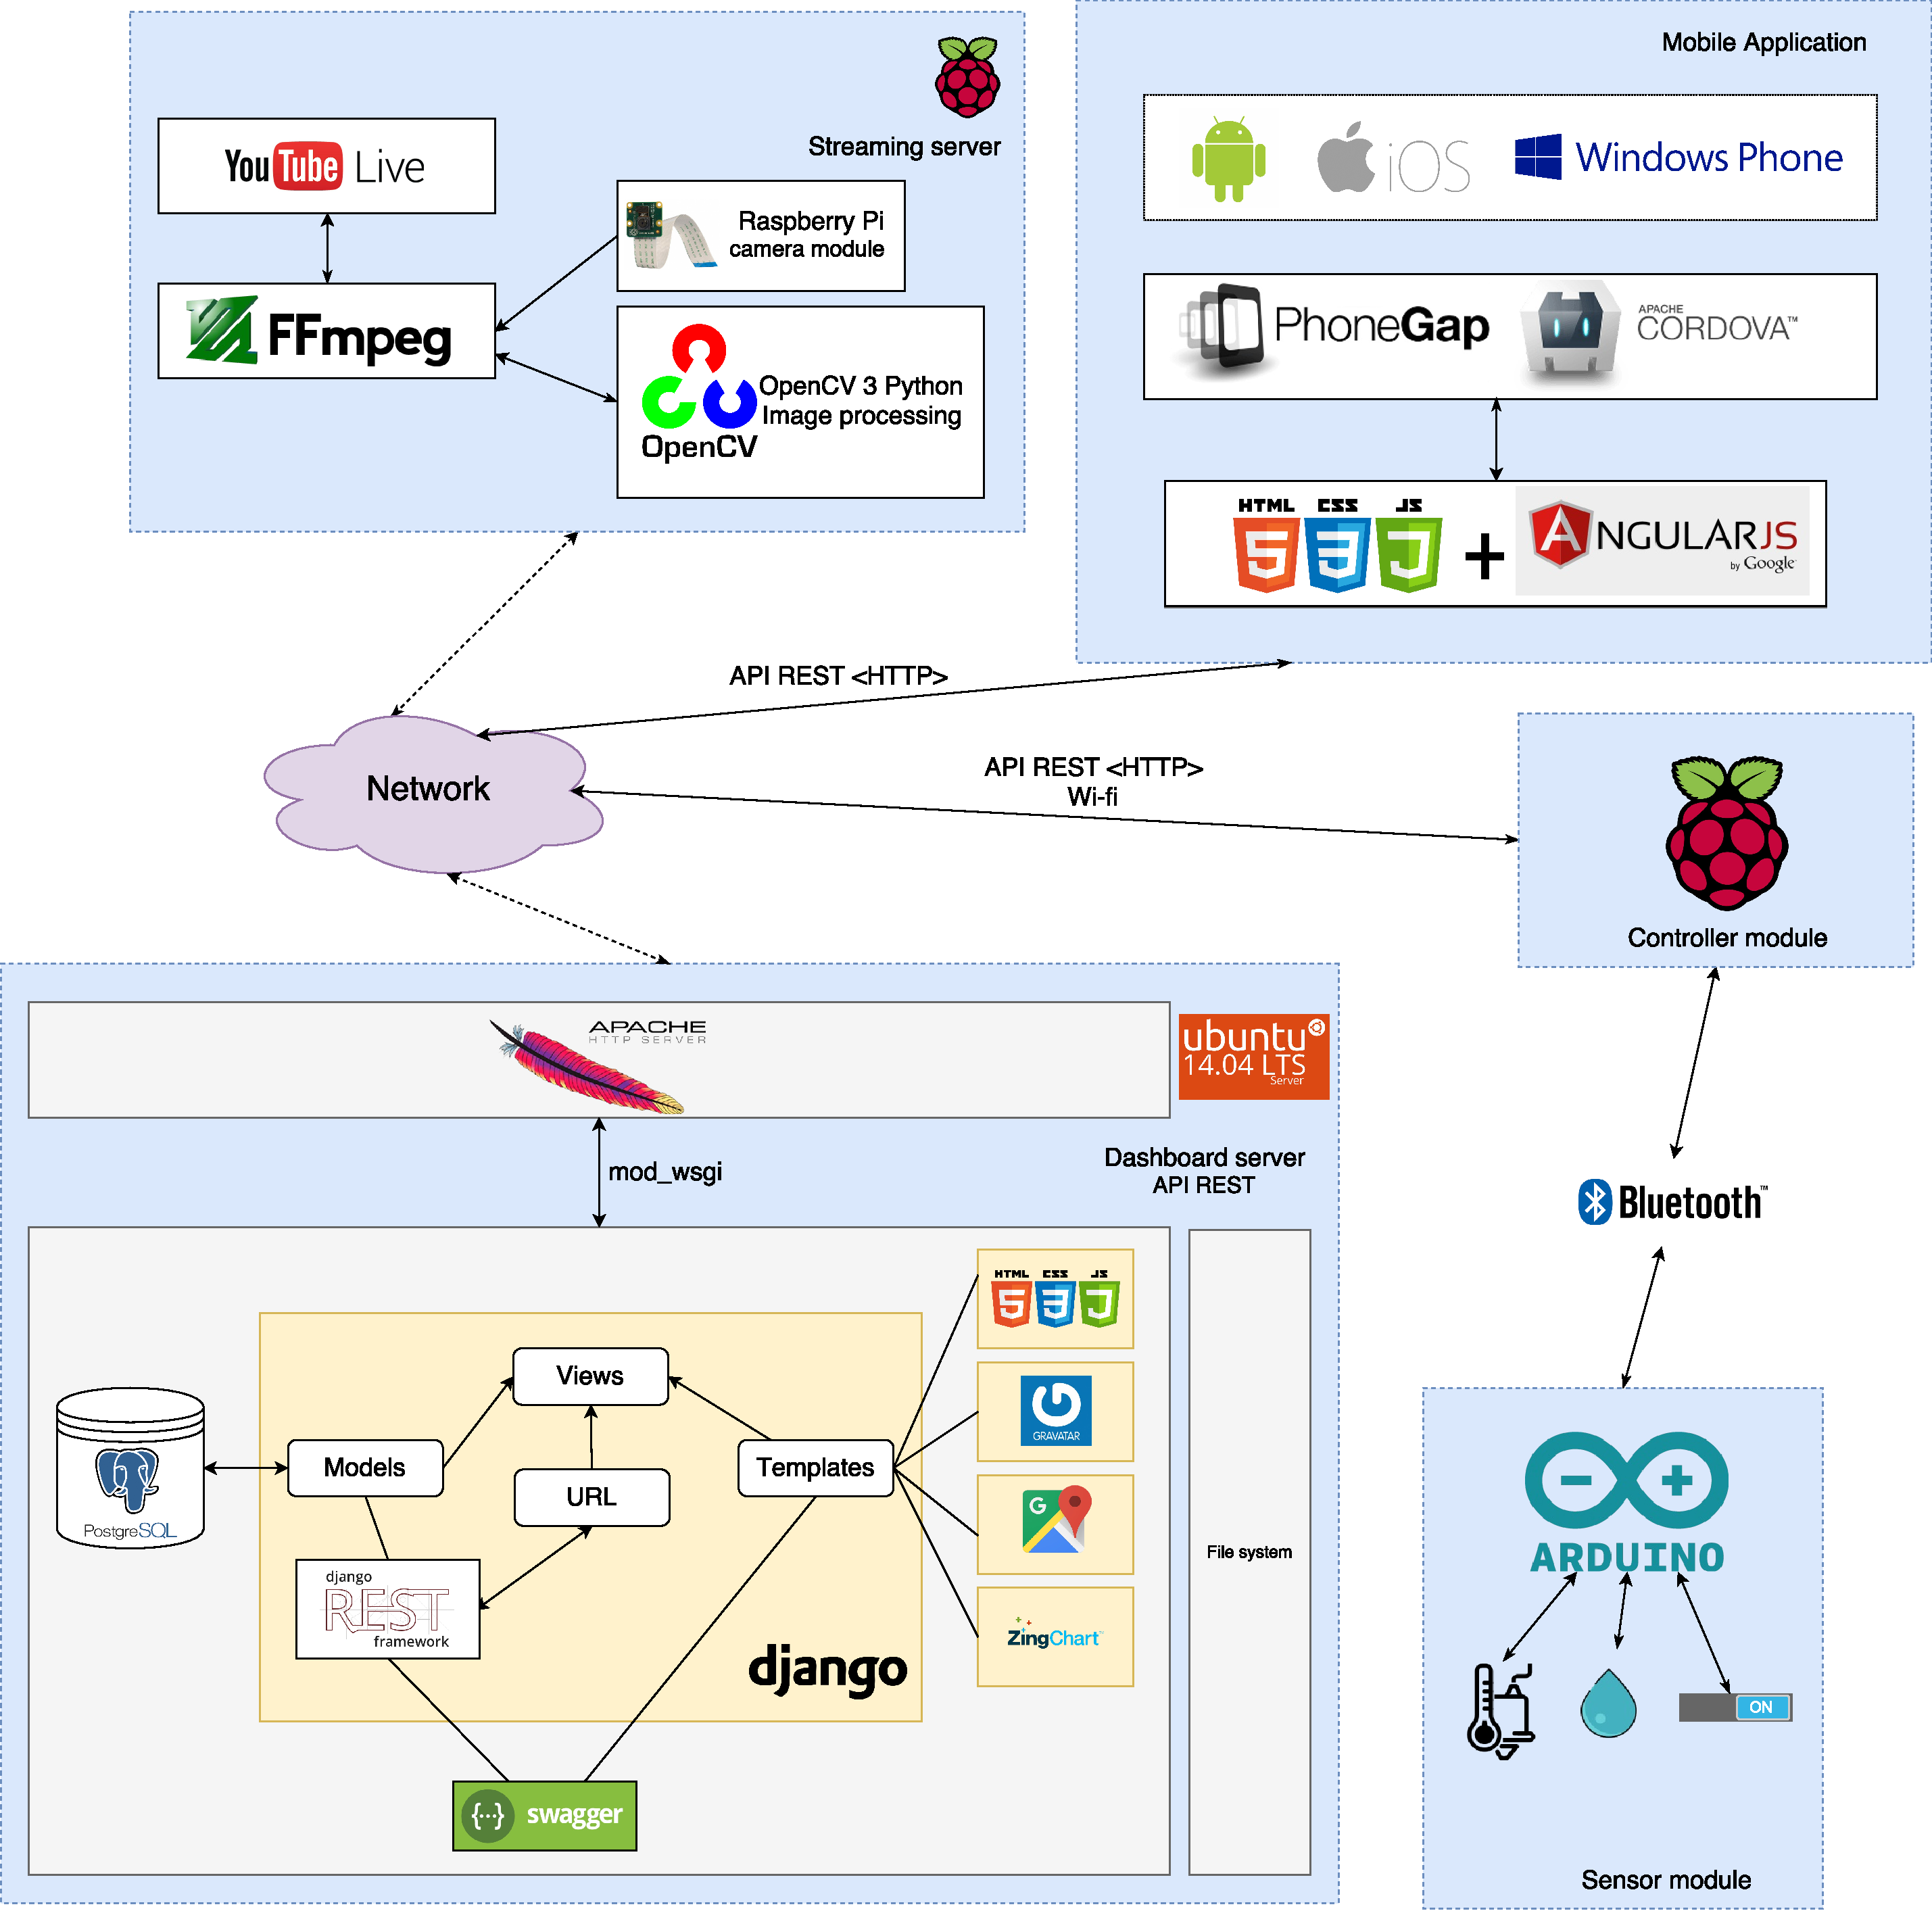
\includegraphics[width=\linewidth]{esquemas/arquitetura-final.pdf}
	\caption{Esquema relacional da estrutura da base de dados}
	\label{esquemarelacional}
\end{figure}








\newpage








\section{Considerações finais}